\documentclass[journal,twoside,web]{ieeecolor}
\usepackage{jsen}
\usepackage{cite}
\usepackage{amsmath,amssymb,amsfonts}
\usepackage{algorithmic}
\usepackage{graphicx}
\usepackage{textcomp}
\usepackage{wrapfig}
\usepackage{dblfloatfix}
\usepackage{bm}
\usepackage{bbm}
\usepackage{siunitx}
\usepackage{makecell}
\usepackage{array}
\usepackage{url}

\usepackage{placeins}

\newcolumntype{C}[1]{>{\centering\arraybackslash}p{#1}}

\definecolor{orange}{rgb}{1, 0.5, 0}
\newcommand{\yzl}[1]{\textcolor{orange}{#1}}

\definecolor{blue}{rgb}{0, 0.5, 1}
\newcommand{\cs}[1]{\textcolor{blue}{#1}}
\newcommand{\hz}[1]{\textcolor{cyan}{#1}}
\newcommand{\fixme}[1]{\textcolor{red}{\textbf{[FIXME: #1]}}}

\newcommand{\mR}{\mathbb{R}}
\DeclareMathOperator*{\mE}{\mathbb{E}}
\DeclareSIUnit{\hertz}{Hz}
\DeclareMathOperator*{\SO}{SO}

% Ensure numbered section/subsection headings keep intended colors
% even when class-level color stack handling is unstable.
\makeatletter
\renewcommand{\thesectiondis}{\textcolor{nblue}{\thesection.}}
\renewcommand{\thesubsectiondis}{\textcolor{subsectioncolor}{\Alph{subsection}.}}
\let\origsection\section
\def\section{\@ifstar\sectionstarcolor\sectioncolor}
\def\sectioncolor#1{\origsection{\textcolor{nblue}{#1}}}
\def\sectionstarcolor#1{\origsection*{#1}}
\let\origsubsection\subsection
\def\subsection{\@ifstar\subsectionstarcolor\subsectioncolorcmd}
\def\subsectioncolorcmd#1{\origsubsection{\textcolor{subsectioncolor}{#1}}}
\def\subsectionstarcolor#1{\origsubsection*{#1}}
\makeatother


\def\BibTeX{{\rm B\kern-.05em{\sc i\kern-.025em b}\kern-.08em
    T\kern-.1667em\lower.7ex\hbox{E}\kern-.125emX}}
\markboth{\journalname, VOL. XX, NO. XX, XXXX 2024}
{Author \MakeLowercase{\textit{et al.}}: Preparation of Papers for IEEE TRANSACTIONS and JOURNALS (May 2024)}
\definecolor{abstractbg}{rgb}{0.89804,0.94510,0.83137}
\setlength{\fboxrule}{0pt}
\setlength{\fboxsep}{0pt}

\begin{document}
\title{LiDAR-Inertial Odometry via Online RBF Terrain Surface Modeling for Legged-Wheel Robots}
\author{Yizhe Liu,
    Chang Shen,
	Han Zhang, Jingchuan Wang, Weidong Chen
\thanks{Yizhe Liu and Chang Shen contributed equally to this work. All the authors are with School of Automation and Intelligent Sensing, Shanghai Jiao Tong University, Institute of Medical Robotics, Shanghai Jiao Tong University, and Key Laboratory of System Control and Information Processing, Ministry of Education, Shanghai 200240, China. Corresponding author: Han Zhang (e-mail: zhanghan\_tc@sjtu.edu.cn}}

\IEEEtitleabstractindextext{%
\fcolorbox{abstractbg}{abstractbg}{%
\begin{minipage}{\textwidth}%
\begin{wrapfigure}[15]{r}{5in}%
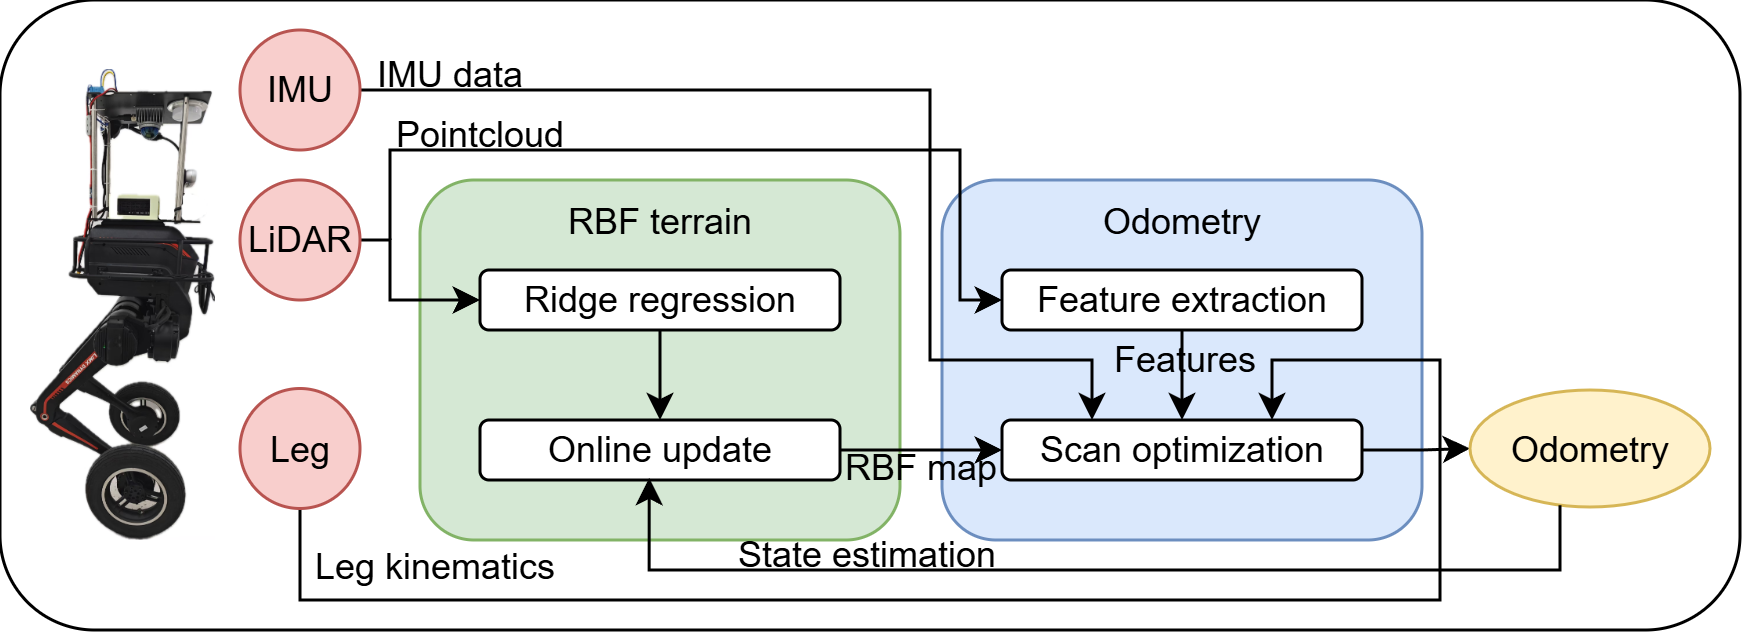
\includegraphics[width=5in]{jsenga.png}%
\end{wrapfigure}%
\begin{abstract}
%An accurate odometry is essential for legged-wheel robots operating in unstructured terrains such as bumpy roads and staircases. Existing methods often suffer from pose drift due to their ignorance of terrain geometry. 
Legged-wheel robots excel at traversing unstructured terrains, including bumpy roads and staircases. However, in such environments, neglecting terrain geometry can lead to severe odometry drifts. In particular, abrupt vertical accelerations caused by uneven surfaces may introduce significant pose errors along the z-axis, thereby degrading both localization and mapping accuracy. To address this issue,
we propose a terrain-aware LiDAR-Inertial odometry (LIO) framework that approximates the terrain using Radial Basis Functions (RBFs) whose centers are adaptively selected and weights are recursively updated.
The resulting smooth terrain manifold enables ``soft constraints" that regularize the odometry optimization and mitigates the $z$-axis pose drift under abrupt elevation changes during robot's maneuver. To ensure the LIO's real-time performance, we further evaluate the RBF-related terms and calculate the inverse of the sparse kernel matrix with GPU parallelization.
Experiments on unstructured terrains demonstrate that our method achieves higher localization accuracy than the baselines, especially in the scenarios that have continuous height changes or sparse features when abrupt height changes occur.
\end{abstract}

\begin{IEEEkeywords}
Simultaneous localization and mapping, 
terrain mapping, LiDAR--Inerial odometry(LIO), legged-wheel robot
\end{IEEEkeywords}
\end{minipage}}}

\maketitle

\definecolor{limegreen}{rgb}{0.2, 0.8, 0.2}
\definecolor{forestgreen}{rgb}{0.13, 0.55, 0.13}
\definecolor{greenhtml}{rgb}{0.0, 0.5, 0.0}

\section{Introduction}\label{sec:intro}
\IEEEPARstart{L}{egged-wheel} robots combine the high mobility of wheeled platforms with the terrain adaptability of legged systems, making them well suited for inspection tasks in complex environments. In practice, they are often required to traverse challenging terrains such as staircases and bumpy roads. However, locomotion over such uneven terrain typically involves abrupt elevation changes, which may induce impulsive velocity variations.
Such jolts pose significant challenges to odometry and often lead to pose estimation drift, particularly along the $z$-axis. This drift arises from the combined effect of inaccurate inertial propagation and insufficient geometric correction. In particular, on rough terrains, abrupt jolts and elevation changes make IMU-based propagation more susceptible to bias and noise accumulation, while LiDAR scan matching may not always provide sufficiently stable constraints on the robot pose. As a result, the corresponding estimation errors can gradually accumulate into noticeable drift.
This issue is particularly critical for legged-wheel robots because they are physically constrained by the terrain during locomotion. Therefore, terrain geometry naturally provides additional geometric constraints on the robot pose, especially on its height and attitude. If such geometry is not explicitly modeled and incorporated into the estimation framework, these constraints cannot be fully exploited to correct the accumulated errors, which in turn degrades both localization and mapping accuracy. Conventional techniques such as IMU deskewing, keyframing, and planar constraints do not fundamentally address this issue, since they reduce motion distortion, sparsify the optimization graph, or impose local flat-ground assumptions, but do not explicitly account for terrain geometry and the wheel–terrain contact relation. Moreover, explicit terrain modeling is also beneficial for downstream tasks such as terrain-aware motion planning and safe traversal over rough terrain.
Earlier studies usually model the terrain using discrete 2.5-D elevation maps. Although such representations can capture the coarse elevation profile of the environment on a grid, they neglect fine-scale height variations within each cell. A smaller grid size may improve geometric fidelity, but 2.5-D elevation maps remain spatially discontinuous and non-differentiable. As a result, they are not well-suited for direct use in gradient-based optimization within odometry frameworks, which motivates the need for a different terrain representation.

To this end, we use Radial Basis Functions (RBFs) to approximate the terrain. Compared with discrete 2.5-D elevation maps, the proposed representation provides a smooth terrain model directly reconstructed from LiDAR point clouds. Based on the moment conditions, we further develop a recursive ridge regression scheme in a Kalman-filter-like manner to update the RBF weights as new observations arrive. In this way, the terrain model can be continuously refined online as the robot moves.
Since the resulting RBF-based terrain approximation defines a smooth manifold with explicitly available gradients, we further introduce terrain-aware soft constraints into the optimization of the LiDAR--Inertial Odometry (LIO) framework. These soft constraints augment the scan-matching objective with an additional terrain-consistency term, thereby improving the robustness of odometry. In particular, when abrupt height changes occur, the manifold constraint helps regularize the robot pose with respect to the approximated terrain surface and suppresses drift along the $z$-axis. In addition, to further improve real-time performance, both the evaluation of the RBF-related terms and the sparse kernel-matrix inversion are implemented using CUDA-based GPU kernels.
To support accurate terrain reconstruction, the LiDAR is mounted in an inverted configuration (see Fig.~\ref{fig:robot-setting}) so as to enlarge its field of view over the ground surface. This design is motivated not only by the need for dense ground observations in the proposed terrain-aware odometry framework, but also by the requirement of reliable ground perception for downstream leg trajectory planning over uneven terrain.

\begin{figure}[!htpb]
  \centering
  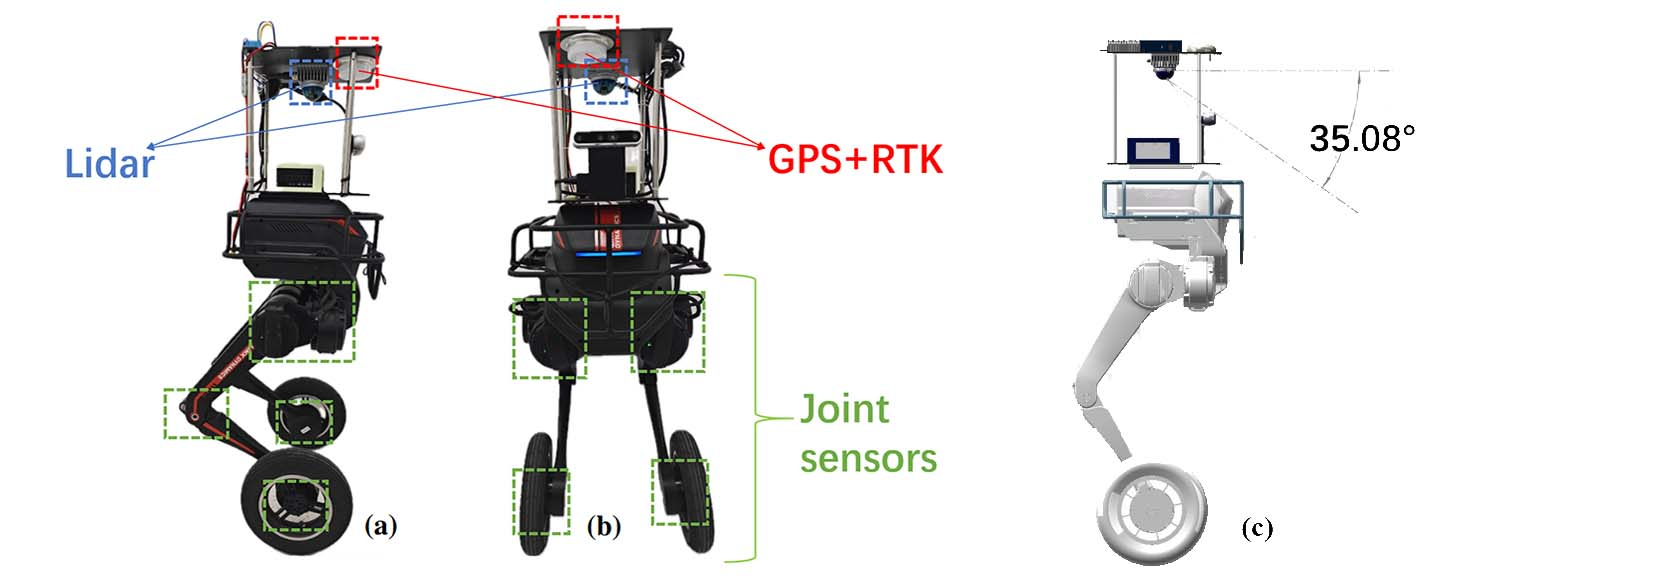
\includegraphics[width=1.0\linewidth]{figure/robot_setting/robot_fov_new.jpg}
  \caption{Robot platform used in our experiments. An inverted Mid-360 LiDAR is mounted on the robot and used in all experiments. The platform is also equipped with a GPS+RTK module (red) and joint sensors (green) for kinematic state estimation. (a) side view, (b) front view, and (c) LiDAR field of view.}
  \label{fig:robot-setting}
\end{figure}

\cs{It is worth emphasizing that the novelty of this work does not lie in using RBF approximation, ridge regression, wheel--terrain contact, or LiDAR--inertial odometry as isolated components. Instead, the key contribution lies in coupling these components into a terrain-aware odometry framework in which the terrain is represented as an online-updated differentiable manifold and is directly used to regularize the pose optimization through wheel--terrain contact geometry. In this way, the terrain model is not only a mapping output or a preprocessing module, but also an active geometric constraint inside the LIO optimization. This design enables the estimator to exploit the physical contact between the wheel-legged platform and the terrain, which is particularly useful for suppressing accumulated vertical drift under abrupt elevation changes.}

To summarize, the main contributions of this work are three-fold:
\begin{itemize}
    \item We propose an RBF-based terrain representation for uneven environments, which provides a smooth and differentiable approximation of the terrain from LiDAR point clouds. Based on moment conditions, a recursive ridge regression scheme is developed to update the RBF weights online as new observations arrive. In addition, an adaptive RBF center selection strategy and GPU parallelization are introduced to improve computational efficiency.
    
    \item \cs{We develop terrain-aware soft constraints that couple the online RBF terrain manifold with the wheel--terrain contact geometry and integrate them into the LIO scan-matching optimization. The proposed formulation uses the reconstructed terrain as an active geometric regularizer for pose estimation, thereby suppressing vertical drift and improving odometry robustness on rough terrain.}
    
    \item We validate the proposed framework through extensive experiments on a legged-wheel robot platform in uneven-terrain scenarios. The proposed method outperforms FAST-LIO2~\cite{fastlio2}, GLIM~\cite{glim}, Leg-KILO~\cite{leg-kilo}, ROLO-SLAM~\cite{roloslam} and Wheel-Legged SLAM~\cite{wl-slam} in challenging environments, especially in scenes with continuous height variations and sparse features. We also release the dataset \footnote{Available at \url{https://zhanghan-tc.github.io/legged_wheel_dataset/}} collected in this study to support future evaluation of SLAM methods for legged-wheel robots.
\end{itemize}

\section{Related Work}

LiDAR--inertial odometry (LIO) has been widely studied in recent years. LOAM \cite{loam} achieves accurate real-time odometry and mapping using LiDAR-only input. Later works, such as LIO-SAM \cite{liosam}, Fast-LIO2 \cite{fastlio2, fastlio}, and GLIM \cite{glim}, further improve robustness and accuracy by tightly coupling LiDAR and IMU measurements. However, these general-purpose LIO frameworks do not explicitly model terrain geometry, and therefore often suffer from pose drift when operating on height-varying or unstructured terrain.

To improve state estimation on legged or wheel-legged platforms, several works exploit kinematic or contact information. Leg-KILO \cite{leg-kilo} incorporates leg kinematics and extracts LiDAR points around the foot contact region to construct local contact-plane constraints. In particular, it assumes that the terrain around each foot contact is approximately flat within a radius of 10\,cm. Wheel-Legged SLAM \cite{wl-slam} similarly integrates the kinematic model of wheel-legged robots to improve LiDAR--inertial SLAM. VILENS \cite{vilen} couples leg odometry with visual, inertial, and LiDAR measurements for quadruped robots, but it does not explicitly construct a continuous terrain model. LIKO \cite{liko} fuses LiDAR, IMU, and kinematic measurements from joint encoders and torque-related sensing on a biped robot, and estimates both the robot state and the foot contact position online. While these methods demonstrate the value of contact and kinematic constraints, they generally rely on local planar approximations, discrete contact events, or accurate contact detection and non-slipping assumptions. However, they do not explicitly construct a continuous and differentiable terrain manifold for direct use in gradient-based LIO optimization. As a result, the associated terrain information is usually introduced only through local planar approximations or discrete contact events, rather than as a smooth function of the robot pose. Consequently, it is difficult for such constraints to provide consistent first-order geometric information throughout the iterative optimization process, which limits their ability to continuously correct height and attitude errors on uneven terrain.
ROLO-SLAM \cite{roloslam} estimates the robot rotation first and then estimates the translation under the rotation constraint. However, for legged-wheel robots operating on uneven terrain, rotation and translation are often strongly coupled due to frequent body tilting. Consequently, such a decoupled strategy may lead to severe drift and degraded robustness.

Beyond contact- and kinematics-based methods, some SLAM systems have also been developed for legged robots from other perspectives. For example, ARS-SLAM \cite{ars-slam} improves spinning-LiDAR SLAM for quadruped robots in large-scale scenarios, while FRL-SLAM \cite{frl-slam} targets lightweight SLAM for quadruped navigation. These methods are relevant to legged-robot SLAM, but they do not focus on terrain-aware LiDAR--inertial estimation with an explicit continuous terrain model.

These limitations motivate the explicit use of terrain geometry in LIO design. To better capture the geometry of uneven environments, elevation mapping has been widely adopted. Early works on robot-centric elevation maps \cite{elevation_map_2014} and probabilistic terrain representations \cite{elevation_map_2018} improve terrain awareness by incorporating elevation uncertainty. Later methods exploit GPU acceleration for real-time elevation mapping \cite{elevation_map_gpu}. Moreover, based on discrete elevation maps, \cite{lio_gc} leverages terrain slope and ground constraints to improve vertical accuracy in LiDAR--inertial odometry. However, elevation maps are defined on fixed-resolution grids and are therefore not spatially differentiable. As a result, the corresponding constraints are typically derived from discretized grids or local planar patches, which yield only piecewise and non-smooth gradient information and are therefore less suitable for gradient-based optimization.

Beyond grid-based elevation maps, \cite{elevation_map_gp} employs Gaussian Process (GP) regression for probabilistic and continuous surface estimation. Although GP-based models provide smooth terrain representations, their computational cost typically scales poorly with the number of measurements, which makes real-time deployment challenging. On the other hand, radial basis functions (RBFs) offer an attractive alternative for surface reconstruction. In particular, RBFs provide continuous and dense terrain models, and have been successfully applied to 3D shape modeling \cite{rbf2001} and digital terrain interpolation from airborne LiDAR data \cite{rbf_air}. Therefore, RBF-based terrain approximation provides a continuous and differentiable representation that can be naturally integrated into optimization-based estimation. Nevertheless, as LiDAR measurements accumulate over time, direct least-squares estimation of the RBF weights becomes computationally expensive. Recursive approaches provide a systematic way to address this issue. In particular, the connection between Recursive Least Squares (RLS) and the Kalman filter has been well established in optimization theory \cite{OptVec}, enabling incremental updates of model parameters as new data arrive. However, this perspective remains largely underexplored in LIO systems.

\cs{Building on these observations, RBF-LIO uses an online RBF terrain function as a differentiable intermediate representation that connects terrain mapping and pose optimization through wheel--terrain contact geometry. The proposed method is related to several lines of prior work, but differs from them in how terrain geometry is represented, updated, and used in state estimation. General-purpose LIO methods such as LOAM, LIO-SAM, Fast-LIO2, and GLIM mainly rely on LiDAR geometric features and inertial propagation, but do not explicitly construct a terrain model that can constrain the robot height and attitude. Contact- or kinematics-aided methods such as Leg-KILO and Wheel-Legged SLAM exploit the robot morphology, but their terrain information is typically introduced through local flatness assumptions, discrete contact constraints, or kinematic consistency, rather than through a continuously differentiable terrain function. Elevation-map-based approaches can encode terrain height, but the grid representation makes the resulting gradients resolution-dependent and less suitable for direct smooth optimization. GP-based terrain models provide continuous surfaces, but their computational cost is less favorable for online LIO when measurements accumulate.}

\cs{In contrast, RBF-LIO uses an RBF terrain function as an intermediate representation that connects terrain mapping and odometry optimization. The RBF model provides continuous height and gradient queries at arbitrary contact locations. The recursive ridge-regression update keeps the terrain representation online and computationally tractable, while the adaptive center selection avoids introducing unsupported or redundant kernels. More importantly, the approximated terrain manifold is coupled with wheel--terrain contact geometry and inserted into the scan-matching optimization as a soft constraint. }

\section{Preliminaries and Problem Formulation}
\label{sec:problem_formulation}

Before introducing the RBF-based terrain approximation, we first formulate the terrain-aware odometry problem considered in this work. This section clarifies why a continuous and differentiable terrain representation is required and how such a terrain model is used in the LiDAR--inertial odometry framework.

At the $k$-th LiDAR frame, let the robot base pose be denoted by
\begin{equation}
    \bm{\eta}_k =
    \left(
    {}^{\mathrm{O}}\mathbf{R}_{\mathrm{B},k},
    {}^{\mathrm{O}}\mathbf{t}_{\mathrm{B},k}
    \right),
\end{equation}
where ${}^{\mathrm{O}}\mathbf{R}_{\mathrm{B},k}\in SO(3)$ and
${}^{\mathrm{O}}\mathbf{t}_{\mathrm{B},k}\in\mathbb{R}^{3}$ denote the rotation matrix and translation vector from the base frame to the world frame, respectively. A standard feature-based LIO front-end estimates $\bm{\eta}_k$ by minimizing point-to-line and point-to-plane residuals extracted from the LiDAR scan. In this work, the scan-matching objective is written as
\begin{equation}
\begin{aligned}
    J_{\mathrm{scan}}(\bm{\eta}_k)
    &=
    \sum_{\mathbf{p}^{e}_{s,k}\in\mathcal{F}^{e}_{k}}
    \left\|
    d_e\left(\bm{\eta}_k;\mathbf{p}^{e}_{s,k}\right)
    \right\|^{2}  \\
    &\quad+
    \sum_{\mathbf{p}^{p}_{s,k}\in\mathcal{F}^{p}_{k}}
    \left\|
    d_p\left(\bm{\eta}_k;\mathbf{p}^{p}_{s,k}\right)
    \right\|^{2},
\end{aligned}
\label{eq:problem_scan_matching}
\end{equation}
where $\mathcal{F}^{e}_{k}$ and $\mathcal{F}^{p}_{k}$ denote the extracted edge and planar feature sets. Moreover, $d_e(\cdot)$ and $d_p(\cdot)$ denote the corresponding point-to-line and point-to-plane residuals. This formulation is effective when sufficient and well-distributed LiDAR geometric features are available. However, for a legged-wheel robot moving on stairs, slopes and grass, the vertical direction can be weakly constrained by scan matching alone. Abrupt body motion over uneven terrain may also degrade inertial propagation, which further leads to accumulated drift along the $z$-axis.

A common way to describe terrain geometry is to use a discrete 2.5-D elevation map,
\begin{equation}
    p_z = h_{\mathrm{grid}}(p_x,p_y).
\end{equation}
Although such a representation is convenient for terrain visualization and navigation, the height value is defined on discrete grid cells. Therefore, its gradient is usually obtained by finite differences and depends on the grid resolution. The resulting geometric constraint is only piecewise smooth and is not ideal for direct use in gradient-based LIO optimization. Another common simplification is to approximate the terrain around a contact point by a local plane,
\begin{equation}
    \mathbf{n}^{\top}\left(\bm{\chi}-\mathbf{p}_0\right)=0,
    \label{eq:problem_local_plane}
\end{equation}
where $\bm{\chi}$ is the contact point, while $\mathbf{n}$ and $\mathbf{p}_0$ denote the local terrain normal and a point on the plane. This model is simple, but it only describes the terrain geometry in a small neighborhood. On stairs, curved slopes, or mixed grass--pathway regions, the local plane may change abruptly and cannot provide a consistent smooth terrain manifold for pose regularization.

These limitations motivate the use of a continuous terrain function
\begin{equation}
    p_z = f(\mathbf{x};\mathbf{w}),
    \qquad
    \mathbf{x}=[p_x,p_y]^{\top},
    \label{eq:problem_terrain_function}
\end{equation}
where $\mathbf{w}$ denotes the terrain model parameters. Such a terrain function should satisfy three requirements. First, it should predict the terrain height at arbitrary horizontal query points. Second, its spatial gradient should be available for constructing smooth residuals and Jacobians. Third, it should be updated online from streaming LiDAR measurements with bounded computational cost.

With this terrain representation, the wheel--terrain contact relation can be used as an additional geometric constraint for pose estimation. For each wheel $j\in\{L,R\}$, let $\bm{\chi}_{j,k}$ denote the corresponding contact point expressed in the world frame. Instead of enforcing the contact relation as a hard constraint, we define a soft manifold residual
\begin{equation}
    \mathbf{r}^{j}_{M}
    =
    \mathbf{r}^{j}_{M}
    \left(
    \bm{\eta}_k,
    \bm{\chi}_{j,k},
    f(\cdot;\mathbf{w})
    \right),
    \label{eq:problem_manifold_residual}
\end{equation}
which measures the consistency among the robot pose, the wheel geometry, and the approximated terrain surface. The terrain-aware pose optimization considered in this work can then be summarized as
\begin{equation}
\begin{aligned}
    \min_{\bm{\eta}_k,\{\bm{\chi}_{j,k}\}}
    \quad
    J_{\mathrm{scan}}(\bm{\eta}_k)
    +
    \lambda_{M}
    \sum_{j\in\{L,R\}}
    \left\|
    \mathbf{r}^{j}_{M}
    \left(
    \bm{\eta}_k,
    \bm{\chi}_{j,k},
    f(\cdot;\mathbf{w})
    \right)
    \right\|^{2},
\end{aligned}
\label{eq:problem_total_cost}
\end{equation}
where $\lambda_{M}$ is the weight of the manifold constraint.

In practice, the problem is solved online in two coupled steps. Given the current pose estimate and the local terrain point cloud, the RBF terrain model is first updated to obtain the smooth function $f(\mathbf{x};\mathbf{w})$. Then, the resulting terrain manifold is queried at the wheel contact locations and introduced into scan matching through the residual $\mathbf{r}^{j}_{M}$.




\section{The RBF-based Terrain Approximation}\label{sec:RBF_approximation}
\cs{Based on the formulation in Sec.~\ref{sec:problem_formulation}, this section introduces the RBF-based terrain approximation method. In particular, we first introduce the RBF approximation model for the terrain and then present the recursive ridge regression used for the weight update. Note that, in this section, the robot's base pose is assumed to be known.}
\subsection{The RBF Approximation Model}\label{sec: RBF_approximation_model}
The RBF approximation is universal \cite{rbf2001}, i.e., given enough centers, it can approximate any continuous function on a compact set to arbitrary accuracy.  
Consequently, the RBF approximation model gives a dense, smooth representation for the terrain.
Compared to 2.5-D elevation maps, the RBF approximation model can predict the height at any arbitrary point within the compact Region of Interest (ROI) $\mathcal{X}$.
Moreover, its spatial gradient can be calculated explicitly at any point, which is essential for solving the optimization problem for the LIO.

To this end, we let the RBF approximation for the terrain be
\begin{equation}
    f(\mathbf{x};\mathbf{w}) = \sum_{i=1}^{N} w_i \, \phi(\lVert \mathbf{x} - \mathbf{c}_i \rVert_2),
    \label{RBF_fml}
\end{equation}
where
\begin{itemize}
    \item \( \mathbf{x} =[p_x,p_y]^\top\in \mathbb{R}^2 \) is a 2D query point in the horizontal plane, and \( f(\mathbf{x};\mathbf{w}) \) denotes the predicted terrain height at the query point;
    \item \( \mathbf{c}_{1:N}:=\{ \mathbf{c}_i = (x_i^c, y_i^c)\in\mathcal{X}\}_{i=1}^{N} \subset \mathbb{R}^2 \) are the RBF center points, which will be selected adaptively based on the distribution of the terrain point cloud;
    \item \(\mathbf{w}:= \{w_i \in \mathbb{R}\}_{i=1}^N \) are the weights of the RBFs;
    \item \( \phi(\cdot) \) is the RBF. In this work, we use the Gaussian kernel, namely,
    \begin{align}
        \phi(r_i) = e^{-\frac{(r_i)^2}{2\sigma^2}}:=\kappa_{\sigma}(\mathbf{x};\mathbf{c}_j),\label{eq:RBF_def}
    \end{align}
    where \( r_i = \lVert \mathbf{x} - \mathbf{c}_i \rVert_2 \) is the Euclidean distance between the query point $\mathbf{x}$ and center $\mathbf{c}_i$, and \( \sigma\in \mR\) is a bandwidth parameter that determines the spatial influence of the kernel.
\end{itemize}
\iffalse
Notably, the model \eqref{RBF_fml} predicts the terrain height as a continuous function of 2D spatial coordinates.
Also foreseeably, the number and placement of the RBF centers will affect the approximation accuracy to great extent.
In particular, to achieve a more accurate approximation, we need to add more centers. But given the fact that there are only a finite number of LiDAR points measured from the terrain, an excessive number of centers will not only increase the computation cost but also lead to numerical instability when estimating the weights.
Moreover, since the exponential function in the Gaussian kernel decays very fast as $r_i$ increases, \cs{most entries of $\mathbf{m}(\mathbf{x}_k^i)$ — a vector of kernel values to be defined in Sec. \ref{sec_LS} — would be almost zero. Consequently, this would lead to an sparse and ill-conditioned information matrix $\mathbf{H}_k$, also to be defined in Sec. \ref{sec_LS}, and affect the approximation accuracy.} Hence the number and the placement of the centers need to be carefully considered to give an accurate approximation of the terrain.
\fi
Notably, the model \eqref{RBF_fml} predicts the terrain height as a continuous function of 2D spatial coordinates. The number and placement of the RBF centers critically affect the approximation quality. In general, more centers improve the representation capability of the model. However, since the terrain is reconstructed from only a finite set of LiDAR measurements, using too many centers increases the computational cost and may also make the weight estimation numerically unstable. Moreover, due to the rapid decay of the Gaussian kernel, a center that is not sufficiently supported by nearby LiDAR points contributes little useful information to the regression. Hence, the number and placement of the centers must be carefully chosen to balance approximation accuracy, numerical stability, and computational efficiency.

\iffalse
\begin{figure}[!htpb]
  \centering
  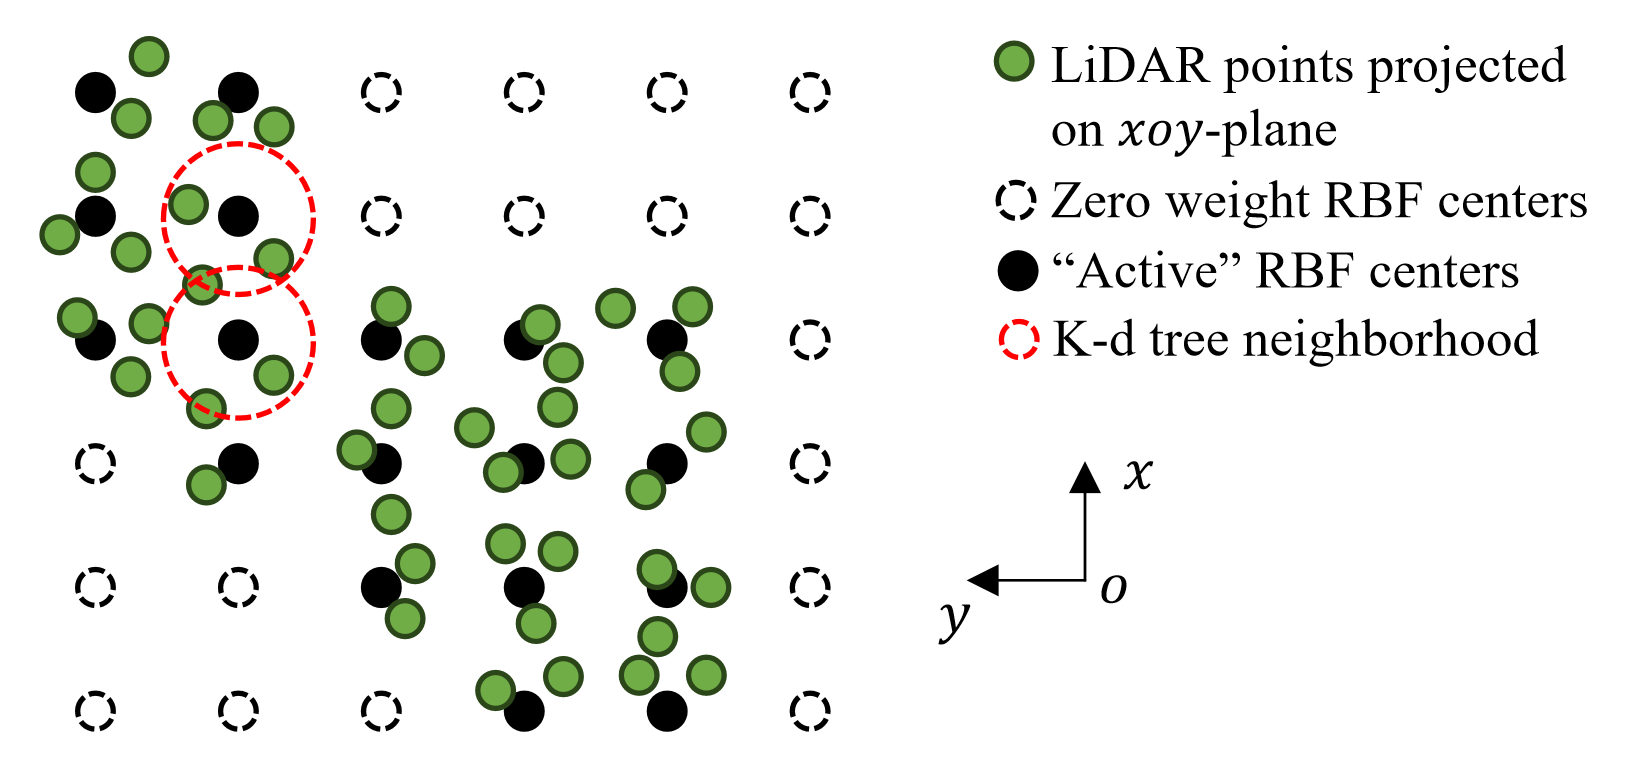
\includegraphics[width=0.9\linewidth]{figure/rbf/kd_tree.png}
  \caption{\yzl{The RBF centers selection strategy. Only the RBF centers that have enough LiDAR points nearby are chosen to be accepted.}}
  \label{fig:kd_tree}
\end{figure}

To this end, we use an adaptive strategy to select the RBF centers as shown in Fig.~\ref{fig:kd_tree}. 
First, we build a k-d tree from the terrain point cloud for efficient neighborhood queries.
Next, we construct the candidate centers on a mesh with a specified resolution in the compact ROI $\mathcal{X}$ of the $xoy$-plane. 
For each candidate center, the k-d tree counts the number of LiDAR points around the candidate center within a radius $r_{kd}$. If the number exceeds a pre-defined threshold, then the candidate center will be accepted. 
\yzl{Moreover, we set $r_{kd}$ equal to the bandwidth parameter $\sigma$ since the  bandwidth parameter represents the spatial influence of each kernel. For practical implementation, we determined that a minimum threshold of 3 LiDAR points is sufficient to achieve reliable results.}
Such a strategy balances the needs for RBF centers' number suppression with the terrain approximation accuracy.
\fi

\begin{figure}[!htpb]
  \centering
  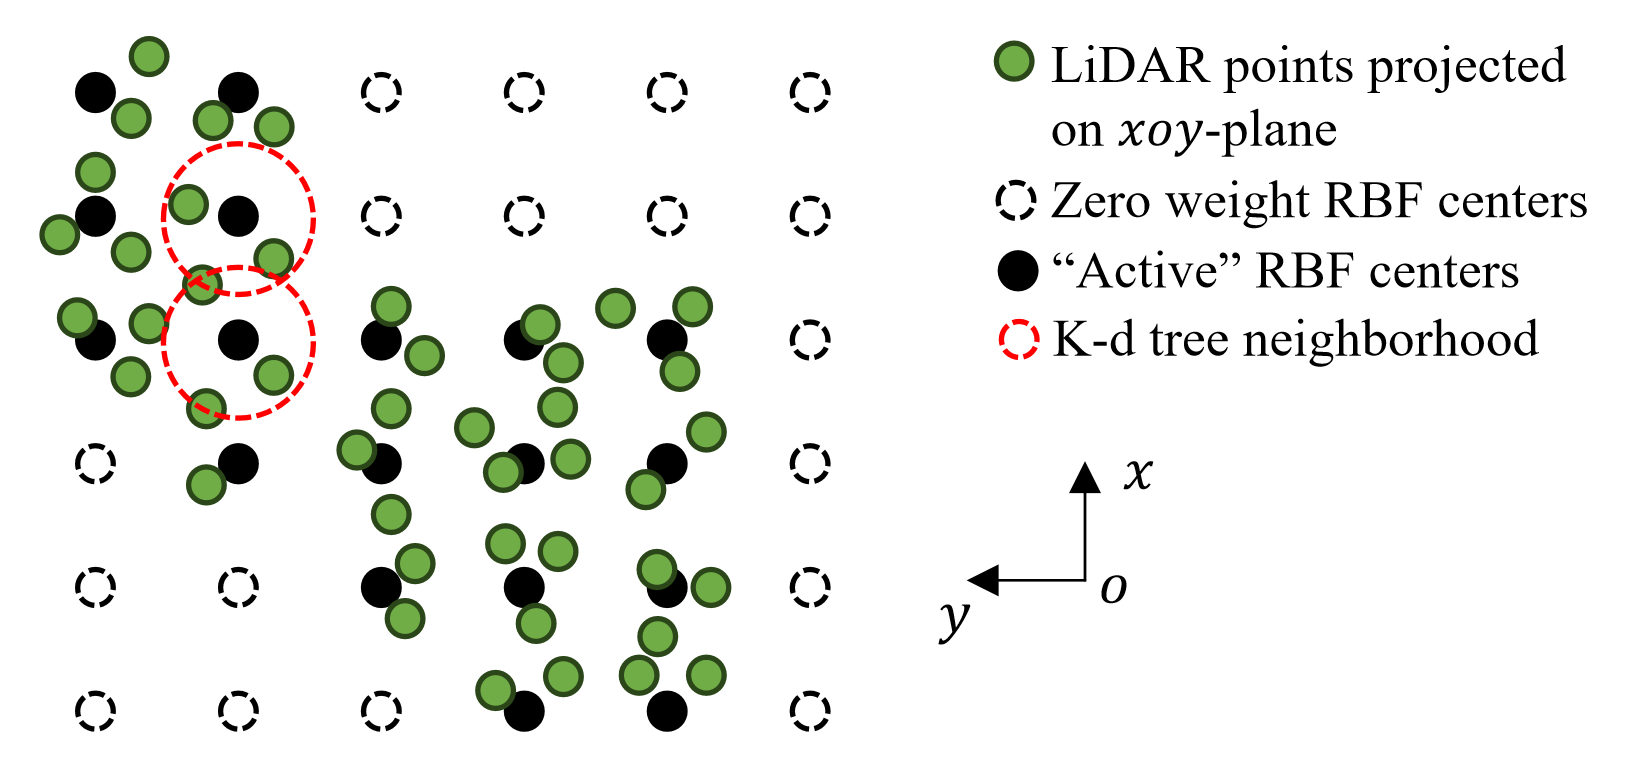
\includegraphics[width=0.9\linewidth]{figure/rbf/kd_tree.png}
  \caption{The RBF center selection strategy illustration on $xoy$-plane. Only candidate centers with sufficient nearby LiDAR support are retained.}
  \label{fig:kd_tree}
\end{figure}

To this end, we use an adaptive strategy to select the RBF centers, as illustrated in Fig.~\ref{fig:kd_tree}. First, we build a k-d tree from the terrain point cloud for efficient neighborhood queries. Next, candidate centers are generated on a mesh with a specified resolution over the compact ROI $\mathcal{X}$ in the $xoy$-plane. For each candidate center, the k-d tree counts the number of LiDAR points within a neighbourhood of radius $r_{kd}$. The candidate center is accepted only if this number exceeds a pre-defined threshold. In our implementation, we set $r_{kd}=\sigma$ so that the neighborhood test is consistent with the effective spatial support of the Gaussian kernel. Empirically, a minimum of three nearby LiDAR points is sufficient to yield reliable center selection. Such a strategy balances approximation accuracy, numerical stability, and computational efficiency.

\subsection{The RBF Weight Estimate by Ridge Regression} \label{sec_LS}

To use \eqref{RBF_fml} to approximate the terrain, we need to estimate the RBF weights. 
When no prior information about the terrain is available, e.g., at initialization, we estimate the RBF weights by solving a ridge regression problem.
More specifically, since the robot's base pose is assumed to be known in this section, 
let $\{ \mathbf{p}^i_k \in \mathbb{R}^3 \}_{i=1}^{M_k}$, $(i=1,\ldots,M_k)$, denote the LiDAR point cloud data at the $k$-th time step expressed in the world frame, where each point \( \mathbf{p}^i_k := [\mathbf{x}_k^{i\top}, p_{z,k}^i]^\top\) are approximately i.i.d. samples of the stochastic vector $\mathbf{p}$, and $\mathbf{x}_k^i:=[p_{x,k}^i, p_{y,k}^i]^\top\in\mR^2$.
In addition, for the purpose of estimation, we model the observed LiDAR points $\mathbf{p}_k^i$, $\forall i,k$, expressed in the world frame, as samples of a stochastic vector $\mathbf{p}$. More specifically, we assume that
\begin{align}\label{eq:stochastic_vector}
    \mathbf{p}:=\begin{bmatrix}
        \mathbf{x}\\p_z
    \end{bmatrix}=\bar{\mathbf{p}}+\bm\epsilon=\begin{bmatrix}\bar{\mathbf{x}}\\\bar{p}_{z}\end{bmatrix}+\begin{bmatrix}
        \epsilon_{\mathbf{x}}\\
        \epsilon_z
    \end{bmatrix},
\end{align}
where $\bar{\mathbf{p}}$ is a stochastic vector of 3D coordinates randomly drawn from the terrain surface expressed in the world frame, $\bar{\mathbf{x}}=[p_{x},p_{y}]^\top$, and $\bm\epsilon\sim\mathcal{N}(0,\sigma_\epsilon^2I)$ denotes the point cloud measurement noise, which is assumed to be independent of $\bar{\mathbf{p}}$.
Further, suppose that \eqref{RBF_fml} approximates the terrain surface well on $\mathcal{X}$, i.e.,
\begin{align}\label{eq:fit_height}
    p_z = \underbrace{\begin{bmatrix}
        \kappa_\sigma(\bar{\mathbf{x}};\mathbf{c}_1)&\cdots &\kappa_\sigma(\bar{\mathbf{x}};\mathbf{c}_N)
    \end{bmatrix}}_{\bm{\Phi}(\bar{\mathbf{x}})^\top}
    \underbrace{\begin{bmatrix}
        w_1\\\vdots\\w_N
    \end{bmatrix}}_{\mathbf{w}}+\epsilon_z,
\end{align}
where the centers $\mathbf{c}_j\in\mathcal{X}$, $j=1,\ldots,N$, and $\mathbf{w}$ is the vector of RBF weights.

Next, recall that our goal is to fit the terrain surface by estimating the RBF weights $\mathbf{w}$. 
However, we do not have access to i.i.d.\ samples of $\bar{\mathbf{x}}$, but only to the noisy observations $\mathbf{x}^i_k$ of $\mathbf{x}$. 
To this end, let $\mathbf{m}(\mathbf{x}):=\mE[\bm\Phi(\bar{\mathbf{x}})\mid\mathbf{x}]$. Since $\epsilon_z$ is independent of $\mathbf{x}$, it holds that
\begin{align}\label{eq:conditional_expectation}
    \mE[p_z|\mathbf{x}]=\mE[\bm\Phi(\mathbf{\bar{x}})^\top\mathbf{w}+\epsilon_z|\mathbf{x}]=\mE[\bm\Phi(\mathbf{\bar{x}})^\top|\mathbf{x}]\mathbf{w}=\mathbf{m}(\mathbf{x})^\top\mathbf{w}.
\end{align}
Therefore, by the tower property of conditional expectation, it follows that
\begin{equation}
\begin{aligned}
    \mE[\mathbf{m}(\mathbf{x})p_z]
    &=\mE\!\left[\mE[\mathbf{m}(\mathbf{x})p_z\mid\mathbf{x}]\right]
    =\mE\!\left[\mathbf{m}(\mathbf{x})\mE[p_z\mid\mathbf{x}]\right]\\
    &=\mE[\mathbf{m}(\mathbf{x})\mathbf{m}(\mathbf{x})^\top]\mathbf{w}.
    \label{eq:moment_equality}
\end{aligned}
\end{equation}
Notably, \eqref{eq:moment_equality} forms a moment equality, from which we obtain the estimator at the $k$-th time step:
\begin{align}
&\hat{\mathbf{w}}_k=\mE[\mathbf{m}(\mathbf{x})\mathbf{m}(\mathbf{x})^\top]^{-1}\mE[\mathbf{m}(\mathbf{x})p_z]\nonumber\\
&\approx (\underbrace{\sum_{t=1}^k\sum_{i=1}^{M_t} \mathbf{m}(\mathbf{x}_t^i)\mathbf{m}(\mathbf{x}_t^i)^\top}_{\mathbf{H}_k})^{-1}
(\underbrace{\sum_{t=1}^k\sum_{i=1}^{M_t}  \mathbf{m}(\mathbf{x}_t^i)p_{z,t}^i}_{\mathbf{b}_k}), \label{eq:RBF_estimator}
\end{align}
where
\begin{align}
    \mathbf{m}(\mathbf{x}_t^i)
    &= \mE[\bm{\Phi}(\bar{\mathbf{x}})\mid\mathbf{x}_t^i]\nonumber\\
    &=\frac{\sigma^2}{\tilde{\sigma}^2}\begin{bmatrix}
        \kappa_{\tilde{\sigma}}(\mathbf{x}_t^i;\mathbf{c}_1) &\cdots & \kappa_{\tilde{\sigma}}(\mathbf{x}_t^i;\mathbf{c}_N)
    \end{bmatrix}^\top,
\end{align}
with $\tilde{\sigma}=\sqrt{\sigma^2+\sigma_\epsilon^2}$, since $\bm\epsilon\sim\mathcal{N}(0,\sigma_\epsilon^2 I)$.
Moreover, \eqref{eq:RBF_estimator} is the unique minimizer of
\begin{align}
    \min_{\mathbf{w}} \sum_{t=1}^k\sum_{i=1}^{M_t}\bigl(p_{z,t}^i-\mathbf{m}(\mathbf{x}_t^i)^\top \mathbf{w}\bigr)^2.
    \label{eq:mm_corresponding_obj_fun}
\end{align}

However, $\mathbf{H}_k$ may be ill-conditioned due to the locality and overlap structure of the RBF kernels, which can significantly affect the approximation accuracy. To address this issue, we add a regularization term to \eqref{eq:mm_corresponding_obj_fun} and solve a ridge regression problem \cite{ridge}, i.e.,
\begin{align}
\min_{\mathbf{w}} \sum_{t=1}^k\sum_{i=1}^{M_t}\bigl(p_{z,t}^i-\mathbf{m}(\mathbf{x}_t^i)^\top \mathbf{w}\bigr)^2 + \lambda \|\mathbf{w}\|^2,
\end{align}
and the corresponding estimator is
\begin{align}
    \hat{\mathbf{w}}^{RG}_k=(\underbrace{\mathbf{H}_k+\lambda I}_{\bm{\mathcal{H}}_k})^{-1}\mathbf{b}_k.
\end{align}
In particular, the ridge penalty $\lambda \|\mathbf{w}\|^2$ mitigates the ill-conditioning of $\mathbf{H}_k$ and numerically stabilizes the least-squares estimate in \eqref{eq:mm_corresponding_obj_fun}. Although this regularization introduces bias, the bias is typically modest in practice, while the reduction in variance may lead to a smaller mean-squared error \cite{ridge}. The choice of $\lambda$ will be further discussed in Sec.~\ref{sec:experiment}.

\subsection{The Recursive RBF Weight Update}\label{recur_RBF}

Recall the terrain approximation model \eqref{RBF_fml}. Since the RBF \eqref{eq:RBF_def} decays exponentially to zero as $r_i$ increases, the kernel $\kappa_\sigma(\mathbf{x};\mathbf{c}_i)$ only captures the terrain geometry in the vicinity of the center $\mathbf{c}_i\in\mathcal{X}$. Therefore, at a new time step $k+1$, only those RBF centers that are sufficiently supported by the newly observed LiDAR points contribute significantly to the update. We refer to such centers as the \emph{active RBF centers}, and the remaining ones as the \emph{inactive RBF centers}.

According to \eqref{eq:RBF_estimator}, the updated estimator from the newly received LiDAR point cloud at time step $k+1$ takes the form
\begin{subequations}
\begin{align}
\hat{\mathbf{w}}_{k+1}^{RG}
&=(\bm{\mathcal{H}}_{k+1})^{-1}(\mathbf{b}_{k}+\mathfrak{m}_{k+1}\mathbf{p}_{z,k+1}),
\label{eq:weights_update}\\
\bm{\mathcal{H}}_{k+1}&=\bm{\mathcal{H}}_k+\mathfrak{m}_{k+1}\mathfrak{m}_{k+1}^\top,
\label{eq:H_update}
\end{align}
\end{subequations}
where $\mathfrak{m}_{k+1}\in\mR^{N\times M_{k+1}}$ and $\mathbf{p}_{z,k+1}\in\mR^{M_{k+1}}$. More specifically,
\begin{subequations}
\begin{align}
    \mathfrak{m}_{k+1}
    &:=\begin{bmatrix}
        \mathbf{m}(\mathbf{x}_{k+1}^1) & \ldots & \mathbf{m}(\mathbf{x}_{k+1}^{M_{k+1}})
    \end{bmatrix}\nonumber\\
    &=\frac{\sigma^2}{\tilde\sigma^2}\begin{bmatrix}
        \kappa_{\tilde\sigma}(\mathbf{x}_{k+1}^1;\mathbf{c}_1) & \cdots & \kappa_{\tilde\sigma}(\mathbf{x}_{k+1}^{M_{k+1}};\mathbf{c}_1)\\
        \vdots & \ddots & \vdots\\
        \kappa_{\tilde\sigma}(\mathbf{x}_{k+1}^1;\mathbf{c}_N) & \cdots & \kappa_{\tilde\sigma}(\mathbf{x}_{k+1}^{M_{k+1}};\mathbf{c}_N)
    \end{bmatrix},
    \label{eq:rbf_kernel}\\
    &\approx
    \frac{\sigma^2}{\tilde\sigma^2}
    \begin{bmatrix}
        \mathbf{0}\\
        \tilde{\mathfrak{m}}_{k+1}\\
        \mathbf{0}
    \end{bmatrix},
    \label{eq:mfk_m_approx}\\
    \mathbf{p}_{z,k+1}
    &:=
    \begin{bmatrix}
        p_{z,k+1}^1 & \cdots & p_{z,k+1}^{M_{k+1}}
    \end{bmatrix}^\top.
\end{align}
\end{subequations}

The approximation \eqref{eq:mfk_m_approx} follows from two facts: the LiDAR scans only cover a local portion of the ROI $\mathcal{X}$, and the kernel $\kappa_{\tilde\sigma}(\mathbf{x};\mathbf{c}_j)$ decays rapidly as the distance between $\mathbf{x}$ and $\mathbf{c}_j$ increases. Hence, most rows of $\mathfrak{m}_{k+1}$ are numerically close to zero, except for those corresponding to the active RBF centers. We refer to these non-negligible rows as the \emph{active rows}. After reordering the centers, the active rows can be grouped into a contiguous block, while the rows corresponding to inactive RBF centers remain approximately zero.
Moreover, in view of \eqref{eq:H_update}, the update induced by $\mathfrak{m}_{k+1}\mathfrak{m}_{k+1}^\top$ only affects the sub-block associated with the active rows. Therefore, $\bm{\mathcal{H}}_k$ exhibits a localized sparse structure, and the recursive update can be organized blockwise after reordering the centers. Furthermore, since $\mathbf{b}_k=\bm{\mathcal{H}}_k\hat{\mathbf{w}}_k^{RG}$, \eqref{eq:weights_update} can be rewritten in a Kalman-filter-style form as
\begin{align}
    \hat{\mathbf{w}}_{k+1}^{RG}
    &= \bm{\mathcal{H}}_{k+1}^{-1}\mathbf{b}_k+\bm{\mathcal{H}}_{k+1}^{-1}\mathfrak{m}_{k+1}\mathbf{p}_{z,k+1}\nonumber\\
    &= \bm{\mathcal{H}}_{k+1}^{-1}\bm{\mathcal{H}}_{k}\hat{\mathbf{w}}_k^{RG}+\bm{\mathcal{H}}_{k+1}^{-1}\mathfrak{m}_{k+1}\mathbf{p}_{z,k+1}\nonumber\\
    &= \bm{\mathcal{H}}_{k+1}^{-1}(\bm{\mathcal{H}}_{k+1}\!-\!\mathfrak{m}_{k+1}\mathfrak{m}_{k+1}^\top)\hat{\mathbf{w}}_k^{RG}
    \!+\!\bm{\mathcal{H}}_{k+1}^{-1}\mathfrak{m}_{k+1}\mathbf{p}_{z,k+1}\nonumber\\
    &= \hat{\mathbf{w}}_k^{RG}
    +\bm{\mathcal{H}}_{k+1}^{-1}\mathfrak{m}_{k+1}
    \bigl[\mathbf{p}_{z,k+1}-\mathfrak{m}_{k+1}^\top\hat{\mathbf{w}}_k^{RG}\bigr].
    \label{eq:kf_w_update}
\end{align}

Due to the sparse structure of $\mathfrak{m}_{k+1}$ in \eqref{eq:mfk_m_approx}, only the block associated with the active RBF centers needs to be updated. After reordering the centers, we partition $\hat{\mathbf{w}}_{k+1}^{RG}$ and $\mathcal{H}_{k+1}^{-1}$ conformably. Then \eqref{eq:kf_w_update} can be written as
\begin{align}
    &\begin{bmatrix}
        \hat{\mathbf{w}}_{1,k+1}^{RG}\\
        \hat{\mathbf{w}}_{2,k+1}^{RG}\\
        \hat{\mathbf{w}}_{3,k+1}^{RG}
    \end{bmatrix}
    =
    \begin{bmatrix}
        \hat{\mathbf{w}}_{1,k}^{RG}\\
        \hat{\mathbf{w}}_{2,k}^{RG}\\
        \hat{\mathbf{w}}_{3,k}^{RG}
    \end{bmatrix}
    +
    \begin{bmatrix}
        \bm{\mathcal{H}}_{1,k+1}^{-1} & & \\
        & \bm{\mathcal{H}}_{2,k+1}^{-1} & \\
        & & \bm{\mathcal{H}}_{3,k+1}^{-1}
    \end{bmatrix}
    \begin{bmatrix}
        \mathbf{0}\\
        \tilde{\mathfrak{m}}_{k+1}\\
        \mathbf{0}
    \end{bmatrix}\nonumber\\
    &\quad\times
    \left[
    \mathbf{p}_{z,k+1}
    -
    \begin{bmatrix}
        \mathbf{0}^\top & \tilde{\mathfrak{m}}_{k+1}^\top & \mathbf{0}^\top
    \end{bmatrix}
    \begin{bmatrix}
        \hat{\mathbf{w}}_{1,k}^{RG}\\
        \hat{\mathbf{w}}_{2,k}^{RG}\\
        \hat{\mathbf{w}}_{3,k}^{RG}
    \end{bmatrix}
    \right]\nonumber\\
    &=
    \begin{bmatrix}
        \hat{\mathbf{w}}_{1,k}^{RG}\\
        \hat{\mathbf{w}}_{2,k}^{RG}
        +\bm{\mathcal{H}}_{2,k+1}^{-1}\tilde{\mathfrak{m}}_{k+1}
        \bigl(\mathbf{p}_{z,k+1}-\tilde{\mathfrak{m}}_{k+1}^\top\hat{\mathbf{w}}_{2,k}^{RG}\bigr)\\
        \hat{\mathbf{w}}_{3,k}^{RG}
    \end{bmatrix}.
    \label{eq:active_rows_weights_update}
\end{align}

Moreover, by Woodbury matrix identity, it holds that
\begin{align}
\bm{\mathcal{H}}_{k+1}^{-1}
&=
\bm{\mathcal{H}}_{k}^{-1}
-
\bm{\mathcal{H}}_{k}^{-1}\mathfrak{m}_{k+1}
\left(I+\mathfrak{m}_{k+1}^\top\bm{\mathcal{H}}_k^{-1}\mathfrak{m}_{k+1}\right)^{-1}
\mathfrak{m}_{k+1}^\top\bm{\mathcal{H}}_{k}^{-1}\nonumber\\
&=
\begin{bmatrix}
    \bm{\mathcal{H}}_{1,k}^{-1} & & \\
    & \bm{\mathcal{H}}_{2,k+1}^{-1} & \\
    & & \bm{\mathcal{H}}_{3,k}^{-1}
\end{bmatrix},
\label{eq:H_inverse_update}
\end{align}
where
\begin{align}
\bm{\mathcal{H}}_{2,k+1}^{-1}\!
:=\!
\bm{\mathcal{H}}_{2,k}^{-1}\!
-\!\bm{\mathcal{H}}_{2,k}^{-1}\tilde{\mathfrak{m}}_{k+1}\!
\left(I\!+\!\tilde{\mathfrak{m}}_{k+1}^\top\bm{\mathcal{H}}_{2,k}^{-1}\tilde{\mathfrak{m}}_{k+1}\right)^{-1}\!\!\!\!
\tilde{\mathfrak{m}}_{k+1}^\top\bm{\mathcal{H}}_{2,k}^{-1}.
\end{align}
In particular, the recursions \eqref{eq:active_rows_weights_update} and \eqref{eq:H_inverse_update} show that only the weights associated with the active RBF centers need to be updated, while the weights corresponding to the inactive RBF centers remain unchanged at the current step, as illustrated in Fig.~\ref{fig:recursive}. Therefore, the recursive update only needs to be applied to the active block, which substantially reduces the computational cost by exploiting the sparse local structure.

\begin{figure}[!htpb]
  \centering
  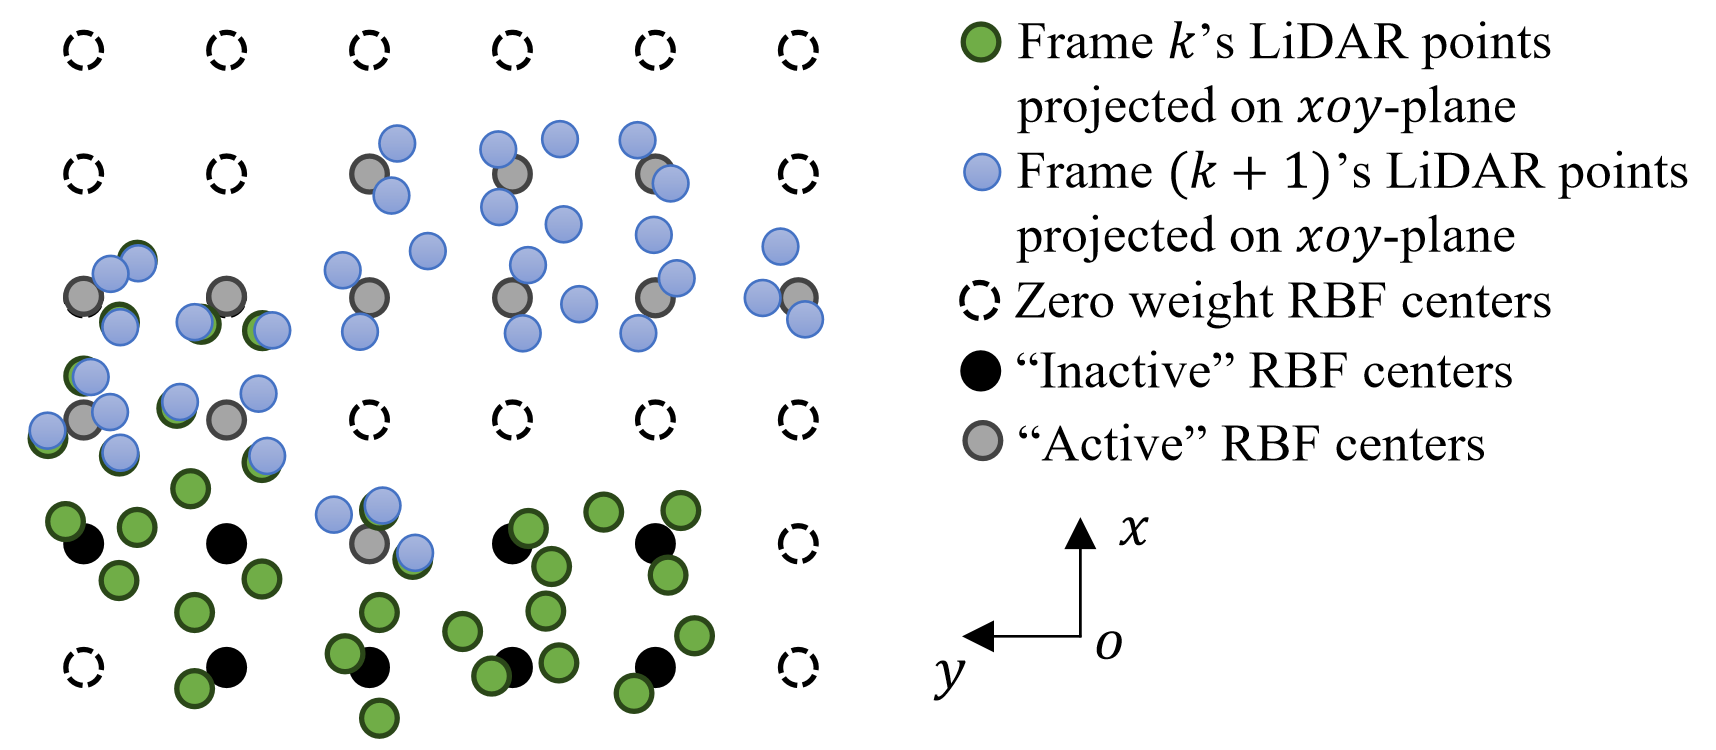
\includegraphics[width=0.9\linewidth]{figure/rbf/recursive.png}
  \caption{Illustration of the recursive RBF weight update on the $xoy$-plane. Only the weights associated with the active RBF centers (gray) are updated, since they are supported by the newly received observations.}
  \label{fig:recursive}
\end{figure}

\section{The LIO with the Manifold Constraint}\label{LIO_MC}
In previous section, we have obtained an approximation of the terrain. Next, we will use such an approximation as the ``soft constraints" in the LIO system to improve the localization accuracy for a legged-wheel robot that maneuvers on the terrain. Such constraints can introduce additional geometric regularization when estimating the robot base pose, particularly in the vertical direction.

\subsection{Leg Kinematics and Wheel–Terrain Contact}
To exploit the manifold constraints, we first characterize the wheel–terrain contact geometry.
To this end, let \( \mathbf{q}_k \) denote the joint configuration at the time step $k$. For each wheel \(j\in\{\text{L},\text{R}\}\), we can easily calculate the wheel centers by the forward kinematics of the leg $\mathbf{h}_j(\mathbf{q})$, and hence the coordinate of wheel center $\bm\xi_j$ expressed in the world frame takes the form
\begin{align}\label{eq:leg_fk}
    \bm\xi_{j}({}^{\text{O}}\mathbf{R}_\text{B}, {}^{\text{O}}\mathbf{t}_{\text{B}}; \mathbf{q}):=\begin{bmatrix}
        \xi_{x,j}\\\xi_{y,j} \\ \xi_{z,j}
    \end{bmatrix}
    ={}^{\text{O}}\mathbf{R}_\text{B} \mathbf{h}_j(\mathbf{q})+{}^{\text{O}}\mathbf{t}_{\text{B}},
\end{align}
where ${}^{\text{O}}\mathbf{R}_\text{B}\in \SO(3)$ and ${}^{O}\mathbf{t}_{\text{B}}\in\mR^3$ denote the rotation matrix and translation vector that transform from the base frame to the world frame.
Similarly, the unit vector along the wheel axis $\mathbf{u}_j$ in the world frame is given by
\begin{align}
    \mathbf{u}_j({}^{\text{O}}\mathbf{R}_\text{B}; \mathbf{q}) = {}^{\text{O}}\mathbf{R}_\text{B}\, \mathbf{g}_j(\mathbf{q}),
\end{align}
 with \(\mathbf{g}_j(\mathbf{q})\) being the axis directions in the base frame derived from leg kinematics.

Moreover, we assume that each wheel admits a unique effective contact point on the terrain at each time step. Let $r$ be the wheel radius and \(\bm{\chi}_j=[\chi_{j,x},\chi_{j,y},\chi_{j,z}]^\top\in\mathbb{R}^3\) denote the contact point between the wheel and the terrain. 
This point must satisfy the following geometric contact constraints:
\begin{subequations}\label{eq:geom_constraints}
\begin{alignat}{2}
&\text{On terrain: }  && \chi_{j,z} - f(\chi_{j,x}, \chi_{j,y}) = 0,\\
&\text{In wheel plane: } && \mathbf{u}_j({}^{\text{O}}\mathbf{R}_\text{B}; \mathbf{q})^\top \mathbf{n}_\omega(\bm{\chi}_j,{}^{\text{O}}\mathbf{R}_\text{B}, {}^{\text{O}}\mathbf{t}_{\text{B}}; \mathbf{q}) = 0,\\
&\text{Radius condition: }  && \|\bm{\chi}_j \!-\! \bm\xi_j({}^{\text{O}}\mathbf{R}_\text{B},\! {}^{\text{O}}\mathbf{t}_{\text{B}}; \mathbf{q})\|^2 \!-\! r^2 \!=\! 0,\\
&\text{Normal collinearity: } && \mathbf{n}_\omega(\bm{\chi}_j,{}^{\text{O}}\mathbf{R}_\text{B}, {}^{\text{O}}\mathbf{t}_{\text{B}}; \mathbf{q}) \times \mathbf{n}_g(\bm{\chi}_j) \!=\! \mathbf{0},
\end{alignat}
\end{subequations}
where \(f\) is the RBF‑based terrain height function defined in \eqref{RBF_fml},
\(\mathbf{n}_g(\bm{\chi}_j)\) is the terrain normal at the contact point computed from the gradient of \(f\),  \(\mathbf{n}_\omega(\bm{\chi}_j,{}^{\text{O}}\mathbf{R}_\text{B}, {}^{\text{O}}\mathbf{t}_{\text{B}}; \mathbf{q})\) is the radial unit vector from the wheel center to the contact point. Specifically,
\begin{subequations}
\begin{align}
&\mathbf{n}_\omega(\bm{\chi}_j,{}^{\text{O}}\mathbf{R}_\text{B}, {}^{\text{O}}\mathbf{t}_{\text{B}}; \mathbf{q}) := \frac{\bm{\chi}_j - \bm\xi_j({}^{\text{O}}\mathbf{R}_\text{B}, {}^{\text{O}}\mathbf{t}_{\text{B}}; \mathbf{q})}{r},\\
&\mathbf{n}_g(\bm{\chi}_j) \!:=\! \frac{1}{\sqrt{1 \!\!+\! \!\bigl(\frac{\partial f}{\partial p_x}\bigr)^2\! \!+\!\! \bigl(\frac{\partial f}{\partial p_y}\bigr)^2}}\!
\begin{bmatrix}
-\frac{\partial f}{\partial p_x}(\chi_{j,x},\chi_{j,y}) \\[4pt]
-\frac{\partial f}{\partial p_y}(\chi_{j,x},\chi_{j,y}) \\[4pt]
1
\end{bmatrix}.
\end{align}
\label{eq:wheel_contact_constraints}
\end{subequations}
We will use \eqref{eq:wheel_contact_constraints} as geometric consistency conditions later on in a soft-constrained optimization framework.

\begin{figure}[!htpb]
    \centering
    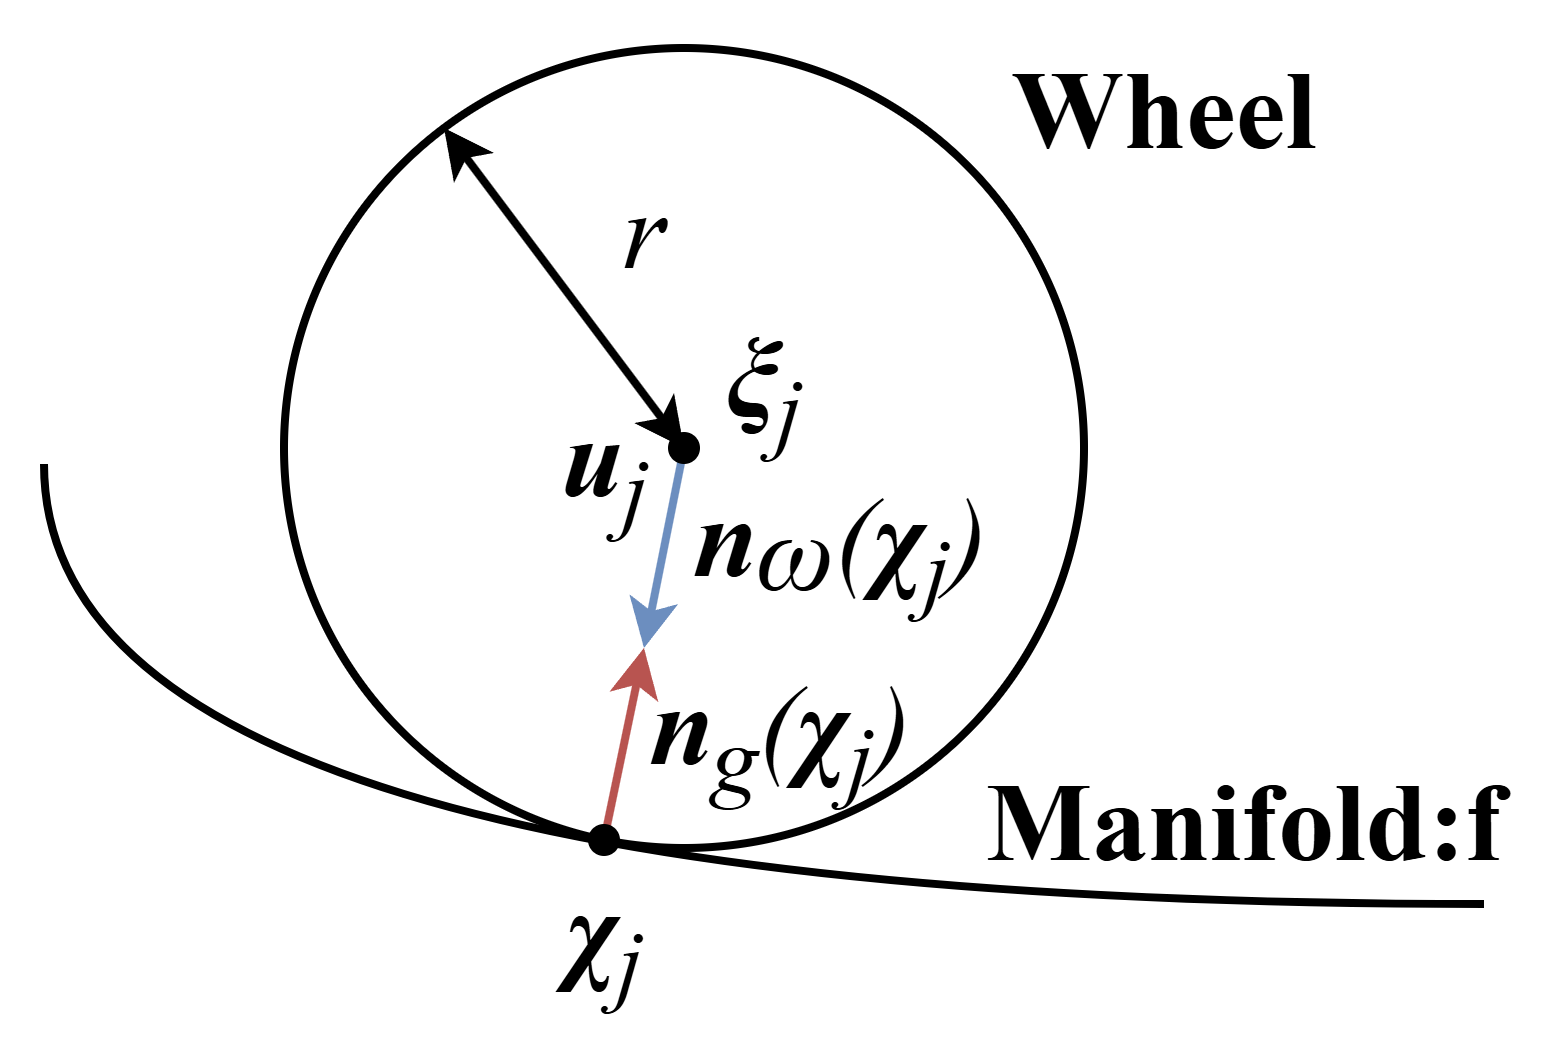
\includegraphics[width=0.5\linewidth]{figure/robot_setting/wheel_new.png}
    \caption{Illustration of wheel–terrain contact.}
    \label{fig:wheel}
\end{figure}

\subsection{IMU Pre-integration}\label{sec:imu-preint}

Due to the relatively low frame rate of LiDAR scans, direct scan matching without a reliable initial guess is prone to convergence issues, especially under abrupt motions. To mitigate this issue, we use an IMU pre-integration module to integrate the high-rate inertial measurements between two consecutive LiDAR frames and provide a motion prior for scan matching.

To this end, let the state estimated by the LIO at time step \(k\) be
\begin{align}
    \bm\eta_k = \bigl({}^{\mathrm{O}}\mathbf{R}_{\mathrm{B},k},\, {}^{\mathrm{O}}\mathbf{t}_{\mathrm{B},k},\, {}^{\mathrm{O}}\mathbf{v}_{\mathrm{B},k},\, \mathbf{b}^a_k,\, \mathbf{b}^g_k \bigr),
\end{align}
where \({}^{\mathrm{O}}\mathbf{R}_{\mathrm{B},k}\) and \({}^{\mathrm{O}}\mathbf{t}_{\mathrm{B},k}\) denote the same pose variables as introduced in \eqref{eq:leg_fk}, \({}^{\mathrm{O}}\mathbf{v}_{\mathrm{B},k}\in\mathbb{R}^3\) is the linear velocity expressed in the world frame, and \(\mathbf{b}^a_k,\mathbf{b}^g_k\in\mathbb{R}^3\) are the accelerometer and gyroscope biases expressed in the local IMU frame, respectively.

Given discrete IMU measurements \(\bigl(\mathbf{a}_i,\boldsymbol{\omega}_i\bigr)\) collected between the \(k\)-th and \((k+1)\)-th LiDAR scans, where \(\mathbf{a}_i\in\mathbb{R}^3\) and \(\boldsymbol{\omega}_i\in\mathbb{R}^3\) denote the linear acceleration and angular velocity measured at time \(t_i\) with sampling interval \(\Delta t_i\), the pre-integrated relative motion can be computed recursively. Let the pre-integration terms be initialized as \(\Delta \mathbf{R}_{k,k}=\mathbf{I}\), \(\Delta \mathbf{v}_{k,k}=\mathbf{0}\), and \(\Delta \mathbf{t}_{k,k}=\mathbf{0}\). Then the propagation from time \(t_i\) to \(t_{i+1}\) is given by
\begin{subequations}
\begin{align}
    \Delta \mathbf{R}_{k,i+1}
    &= \Delta \mathbf{R}_{k,i}\exp\!\left(\lfloor \boldsymbol{\omega}_i-\mathbf{b}^g_k \rfloor_\times \Delta t_i\right),\\
    \Delta \mathbf{v}_{k,i+1}
    &= \Delta \mathbf{v}_{k,i}
    + \Delta \mathbf{R}_{k,i}\bigl(\mathbf{a}_i-\mathbf{b}^a_k\bigr)\Delta t_i+\Delta t_i \mathbf{g},\\
    \Delta \mathbf{t}_{k,i+1}
    &= \Delta \mathbf{t}_{k,i}
    + \Delta \mathbf{v}_{k,i}\Delta t_i
    + \tfrac{1}{2}\Delta \mathbf{R}_{k,i}\bigl(\mathbf{a}_i-\mathbf{b}^a_k\bigr)\Delta t_i^2\nonumber\\
    &\quad +\frac{1}{2}\mathbf{g}\Delta t_i^2.
\end{align}
\end{subequations}
Here, $\mathbf{g}$ denotes the gravity vector in world frame, \(\exp(\cdot)\) denotes the matrix exponential on the Lie algebra \(\mathfrak{so}(3)\), and \(\lfloor\cdot\rfloor_\times\) maps a vector in \(\mathbb{R}^3\) to its corresponding skew-symmetric matrix in \(\mathfrak{so}(3)\). The pre-integrated quantities over the interval \([t_k,t_{k+1}]\) are obtained when \(t_i=t_{k+1}\), and are then used to initialize the scan-matching optimization in the LIO framework.

\subsection{The Manifold Constraints}

We assume that the wheels maintain firm contact with the terrain. Accordingly, for each wheel \(j\in\{\mathrm{L},\mathrm{R}\}\), we define a manifold residual vector by stacking the three scalar contact constraints together with the vector-valued normal-collinearity residual:
\begin{align}\label{eq:residual_manifold_left_wheel}
    \mathbf{r}_{\mathcal{M}}^{j}(\bm\eta_k, \bm{\chi}_j)
    \!&:=\!\!
    \begin{bmatrix}
        r_{j,1}\\[2pt]
        r_{j,2}\\[2pt]
        r_{j,3}\\[2pt]
        \mathbf{r}_{j,4}
    \end{bmatrix}
    \!\!=\!\!
    \begin{bmatrix}
        \chi_{j,z} - f(\chi_{j,x},\chi_{j,y})\\[2pt]
        \mathbf{u}_j({}^{\mathrm{O}}\mathbf{R}_\mathrm{B}; \mathbf{q})^\top
        \mathbf{n}_\omega(\bm{\chi}_j,\!\!{}^{\mathrm{O}}\mathbf{R}_\mathrm{B},\!\! {}^{\mathrm{O}}\mathbf{t}_{\mathrm{B}}; \mathbf{q})\\[2pt]
        \|\bm{\chi}_j - \bm\xi_j({}^{\mathrm{O}}\mathbf{R}_\mathrm{B}, {}^{\mathrm{O}}\mathbf{t}_{\mathrm{B}}; \mathbf{q})\|^2 - r^2\\[2pt]
        \mathbf{n}_\omega(\bm{\chi}_j,{}^{\mathrm{O}}\mathbf{R}_\mathrm{B}, {}^{\mathrm{O}}\mathbf{t}_{\mathrm{B}}; \mathbf{q})
        \times
        \mathbf{n}_g(\bm{\chi}_j)
    \end{bmatrix}\nonumber\\
    &\approx \mathbf{0}.
\end{align}

Next, we incorporate the manifold residuals into the scan-matching optimization. Our LIO framework follows the front-end structure of LIO-SAM \cite{liosam}. In particular, the IMU pre-integration module introduced in Sec.~\ref{sec:imu-preint} is used to provide motion priors between consecutive LiDAR frames, and the associated factor graph is used to update the accelerometer and gyroscope biases.

The scan matching adopted in this work follows the feature-based ICP formulation in LOAM \cite{loam} and LIO-SAM \cite{liosam}. To initialize the ICP optimization, we use the IMU pre-integration between two consecutive frames to estimate the relative motion, which is then composed with the global pose of the previous frame to generate an initial guess for the current frame. More specifically, the scan-matching cost is given by
\begin{equation}
\begin{aligned}
    J_{\mathrm{scan}}(\bm\eta_k)
    &=
    \sum_{\mathbf{p}^e_{s,k}\in\mathcal{F}^e_k}
    \left\|
    \mathbf{d}_e({}^{\mathrm{O}}\mathbf{R}_{\mathrm{B},k},{}^{\mathrm{O}}\mathbf{t}_{\mathrm{B},k};\mathbf{p}^e_{s,k})
    \right\|^2\\
    &\quad+
    \sum_{\mathbf{p}^p_{s,k}\in\mathcal{F}^p_k}
    \left\|
    \mathbf{d}_p({}^{\mathrm{O}}\mathbf{R}_{\mathrm{B},k},{}^{\mathrm{O}}\mathbf{t}_{\mathrm{B},k};\mathbf{p}^p_{s,k})
    \right\|^2,
\end{aligned}
\end{equation}
with respect to \({}^{\mathrm{O}}\mathbf{R}_{\mathrm{B},k}\) and \({}^{\mathrm{O}}\mathbf{t}_{\mathrm{B},k}\), where \(\mathcal{F}^e_k\) and \(\mathcal{F}^p_k\) denote the sets of edge and planar features in the LiDAR scan at time step \(k\). Here, \(\mathbf{p}^e_{s,k}\) and \(\mathbf{p}^p_{s,k}\) denote the \(s\)-th edge and planar feature points extracted from the scan, while \(\mathbf{d}_e(\cdot)\) and \(\mathbf{d}_p(\cdot)\) are the corresponding point-to-line and point-to-plane residuals.

We then incorporate the manifold residuals into the scan-matching objective as soft constraints for pose regularization. The corresponding manifold cost is defined as
\begin{equation}\label{eq:J_M_new}
    J_{\mathcal{M}}(\bm\eta_k,\bm\chi_j)
    =
    \sum_{j\in\{\mathrm{L},\mathrm{R}\}}
    \left\|
    \mathbf{r}_{\mathcal{M}}^j(\bm\eta_k,\bm\chi_j)
    \right\|^2,
\end{equation}
where the contact points $\bm\chi_j$'s are jointly optimized with the pose variables $\bm\eta_k$ in the manifold-constraint term
Therefore, the total cost function takes the form
\begin{equation}\label{eq:cost_fn}
    J_{\mathrm{total}}(\bm\eta_k,\bm\chi_j)
    =
    J_{\mathrm{scan}}(\bm\eta_k)
    +
    J_{\mathcal{M}}(\bm\eta_k,\bm\chi_j).
\end{equation}
In particular, we minimize \eqref{eq:cost_fn} using the Levenberg--Marquardt algorithm \cite{LM_algo}. Since the Jacobians of the point-to-line and point-to-plane residuals have been discussed in detail in \cite{liosam}, we only derive the Jacobian of the newly introduced manifold residual \(\mathbf{r}_{\mathcal{M}}^j(\bm{\eta}_k,\bm{\chi}_j)\) here. In the Levenberg--Marquardt solver, this residual is linearized around the current estimate with respect to the local pose increment and the contact-point increment. Accordingly, for each wheel, we define the joint increment vector as
\[
\delta \mathbf{x}_j
=
\begin{bmatrix}
\delta \boldsymbol{\eta}\\
\delta \bm{\chi}_j
\end{bmatrix},
\qquad
\delta \boldsymbol{\eta}
=
\begin{bmatrix}
\delta \boldsymbol{\theta}\\
\delta \mathbf{t}
\end{bmatrix},
\]
where \(\delta \boldsymbol{\eta}\) denotes the local increment of the base pose. The corresponding Jacobian takes the block form
\begin{equation}\label{J_i}
\mathbf{J}_j
=
\frac{\partial \mathbf{r}_{\mathcal{M}}^j}{\partial \delta \mathbf{x}_j}
=
\begin{bmatrix}
\frac{\partial \mathbf{r}_{\mathcal{M}}^j}{\partial \delta \boldsymbol{\theta}} &
\frac{\partial \mathbf{r}_{\mathcal{M}}^j}{\partial \delta \mathbf{t}} &
\frac{\partial \mathbf{r}_{\mathcal{M}}^j}{\partial \delta \bm{\chi}_j}
\end{bmatrix}.
\end{equation}
Using a right-perturbation model for the rotation increment \(\delta\boldsymbol{\theta}\), the derivatives of the wheel center and wheel-axis direction with respect to the pose increments are
\begin{equation}
\begin{aligned}
\frac{\partial \bm{\xi}_j}{\partial \delta\boldsymbol{\theta}}
&=
-{}^{\mathrm{O}}\mathbf{R}_\mathrm{B}\lfloor\mathbf{h}_j(\mathbf{q})\rfloor_{\times},
\qquad
\frac{\partial \bm{\xi}_j}{\partial \delta\mathbf{t}}
=
\mathbf{I}_3,\\
\frac{\partial \mathbf{u}_j}{\partial \delta\boldsymbol{\theta}}
&=
-\lfloor\mathbf{u}_j\rfloor_{\times}{}^{\mathrm{O}}\mathbf{R}_\mathrm{B},
\qquad
\frac{\partial \mathbf{u}_j}{\partial \delta\mathbf{t}}
=
\mathbf{0}.
\end{aligned}
\end{equation}

With these preliminaries, we derive the Jacobian blocks for each residual component in \eqref{eq:residual_manifold_left_wheel}. Let $\mathbf{d}_j := \bm{\chi}_j - \bm{\xi}_j$.
It follows that
\begin{itemize}
\item \textbf{On terrain:}
$r_{j,1} = \chi_{j,z} - f(\chi_{j,x},\chi_{j,y})$.
Its Jacobian takes the form
\begin{align}\label{eq:manidolf_grad_detail1}
\frac{\partial r_{j,1}}{\partial \delta\boldsymbol{\theta}}
\!=\!
\mathbf{0}_{1\times 3},
\frac{\partial r_{j,1}}{\partial \delta\mathbf{t}}
\!=\!
\mathbf{0}_{1\times 3},
\frac{\partial r_{j,1}}{\partial \delta\bm{\chi}_j}
\!=\!
\begin{bmatrix}
-\frac{\partial f}{\partial x} &
-\frac{\partial f}{\partial y} &
1
\end{bmatrix}.
\end{align}

\item \textbf{In wheel plane:}
$r_{j,2} = \mathbf{u}_j({}^{\text{O}}\mathbf{R}_\text{B}; \mathbf{q})^\top \mathbf{n}_\omega(\bm{\chi}_j,\!\!{}^{\text{O}}\mathbf{R}_\text{B},\!\! {}^{\text{O}}\mathbf{t}_{\text{B}}; \mathbf{q})$.

Since \(\mathbf{n}_\omega=\mathbf{d}_j/r\), it follows that
\begin{equation}
\begin{aligned}\label{eq:manidolf_grad_detail2}
\frac{\partial r_{j,2}}{\partial \delta\boldsymbol{\theta}}
&\!=\!
\frac{1}{r}
\left(
\mathbf{u}_j^\top {}^{\mathrm{O}}\mathbf{R}_\mathrm{B}\lfloor\mathbf{h}_j(\mathbf{q})\rfloor_{\times}
\!-\!
\mathbf{d}_j^\top \lfloor\mathbf{u}_j\rfloor_{\times}{}^{\mathrm{O}}\mathbf{R}_\mathrm{B}
\right),\\
\frac{\partial r_{j,2}}{\partial \delta\mathbf{t}}
&\!=\!
-\frac{\mathbf{u}_j^\top}{r},
\qquad
\frac{\partial r_{j,2}}{\partial \delta\bm{\chi}_j}
=
\frac{\mathbf{u}_j^\top}{r}.
\end{aligned}
\end{equation}

\item \textbf{Radius condition:}
$
r_{j,3}
=
\|\bm{\chi}_j-\bm{\xi}_j({}^{\mathrm{O}}\mathbf{R}_\mathrm{B},{}^{\mathrm{O}}\mathbf{t}_{\mathrm{B}};\mathbf{q})\|^2-r^2$.
Its Jacobian takes the form
\begin{equation}
\begin{aligned}\label{eq:manidolf_grad_detail3}
\frac{\partial r_{j,3}}{\partial \delta\boldsymbol{\theta}}
&=
2\,\mathbf{d}_j^\top {}^{\mathrm{O}}\mathbf{R}_\mathrm{B}\lfloor\mathbf{h}_j(\mathbf{q})\rfloor_{\times},\\
\frac{\partial r_{j,3}}{\partial \delta\mathbf{t}}
&=
-2\,\mathbf{d}_j^\top,
\qquad
\frac{\partial r_{j,3}}{\partial \delta\bm{\chi}_j}
=
2\,\mathbf{d}_j^\top.
\end{aligned}
\end{equation}

\item \textbf{Normal collinearity:}
$
\mathbf{r}_{j,4}
\!\!=\!\!
\mathbf{n}_\omega(\bm{\chi}_j,{}^{\mathrm{O}}\mathbf{R}_\mathrm{B},{}^{\mathrm{O}}\mathbf{t}_{\mathrm{B}};\mathbf{q})
\!\!\times\!\!
\mathbf{n}_g(\bm{\chi}_j).
$
First, the derivatives of \(\mathbf{n}_\omega\) take the form
\begin{align}\label{eq:manidolf_grad_detail4}
\frac{\partial \mathbf{n}_\omega}{\partial \delta\boldsymbol{\theta}}
&\!=\!
\frac{1}{r}{}^{\mathrm{O}}\mathbf{R}_\mathrm{B}\lfloor\mathbf{h}_j(\mathbf{q})\rfloor_{\times},
\frac{\partial \mathbf{n}_\omega}{\partial \delta\mathbf{t}}
\!=\!
-\frac{1}{r}\mathbf{I}_3,
\frac{\partial \mathbf{n}_\omega}{\partial \delta\bm{\chi}_j}
\!=\!
\frac{1}{r}\mathbf{I}_3.
\end{align}
On the other hand, let
\begin{equation}
\begin{aligned}
\mathbf{g}_f\!\!:=\!\!
\begin{bmatrix}
-\frac{\partial f}{\partial p_x}(\chi_{j,x},\chi_{j,y}) \\[4pt]
-\frac{\partial f}{\partial p_y}(\chi_{j,x},\chi_{j,y}) \\[4pt]
1
\end{bmatrix},
\mathbf{H}_f\!\!
:=\!\!
\begin{bmatrix}
-\frac{\partial^2 f}{\partial p_x^2} & -\frac{\partial^2 f}{\partial p_x\partial p_y} & 0\\
-\frac{\partial^2 f}{\partial p_y\partial p_x} & -\frac{\partial^2 f}{\partial p_y^2} & 0\\
0 & 0 & 0
\end{bmatrix}.
\end{aligned}
\end{equation}
Then it holds that
$\frac{\partial \mathbf{n}_g}{\partial \delta\bm{\chi}_j}
=
\frac{1}{\|\mathbf{g}_f\|_2}
\bigl(\mathbf{I}_3-\mathbf{n}_g\mathbf{n}_g^\top\bigr)\mathbf{H}_f$.
Applying the product rule for cross products yields
\begin{equation}
\begin{aligned}\label{eq:manidolf_grad_detail5}
&\frac{\partial \mathbf{r}_{j,4}}{\partial \delta\boldsymbol{\theta}}
\!=\!
-\lfloor\mathbf{n}_g\rfloor_{\times}
\frac{\partial \mathbf{n}_\omega}{\partial \delta\boldsymbol{\theta}}
\!=\!
-\frac{1}{r}
\lfloor\mathbf{n}_g\rfloor_{\times}
{}^{\mathrm{O}}\mathbf{R}_\mathrm{B}
\lfloor\mathbf{h}_j(\mathbf{q})\rfloor_{\times},\\
&\frac{\partial \mathbf{r}_{j,4}}{\partial \delta\mathbf{t}}
\!=\!
-\lfloor\mathbf{n}_g\rfloor_{\times}
\frac{\partial \mathbf{n}_\omega}{\partial \delta\mathbf{t}}
\!=\!
\frac{1}{r}\lfloor\mathbf{n}_g\rfloor_{\times},\\
&\frac{\partial \mathbf{r}_{j,4}}{\partial \delta\bm{\chi}_j}
\!=\!
-\lfloor\mathbf{n}_g\rfloor_{\times}
\frac{\partial \mathbf{n}_\omega}{\partial \delta\bm{\chi}_j}
+
\lfloor\mathbf{n}_\omega\rfloor_{\times}
\frac{\partial \mathbf{n}_g}{\partial \delta\bm{\chi}_j}\\
&=\!
-\frac{1}{r}\lfloor\mathbf{n}_g\rfloor_{\times}
\!+\!
\frac{1}{\|\mathbf{g}_f\|_2}
\lfloor\mathbf{n}_\omega\rfloor_{\times}
\bigl(\mathbf{I}_3\!-\!\mathbf{n}_g\mathbf{n}_g^\top\bigr)\mathbf{H}_f.
\end{aligned}
\end{equation}
\end{itemize}

All these Jacobian blocks are assembled into the full matrix \(\mathbf{J}_j\) in \eqref{J_i}. The overall Jacobian of the manifold cost \(J_{\mathcal{M}}\) is then obtained by stacking the contributions from both wheels.

\section{GPU Acceleration}

The proposed LIO framework contains several computationally intensive modules that are highly amenable to GPU parallelization. Consequently, GPU acceleration can be exploited to improve the real-time performance of the overall system. In particular, two modules benefit the most from GPU implementation:
\begin{enumerate}
    \item \textbf{Evaluation of RBF-related terms.} 
    The evaluation of the RBF terrain model involves computing exponential terms for a large number of center--point pairs. This operation is highly parallelizable and is therefore offloaded to the GPU to exploit data-level parallelism. In our implementation, both the matrix--vector multiplication in the terrain height estimation \eqref{eq:fit_height} and the entries of the RBF kernel matrix in \eqref{eq:rbf_kernel} are computed in parallel on the GPU.
    In addition, evaluating the manifold soft constraints requires both the residuals in \eqref{eq:residual_manifold_left_wheel} for the left and right wheel contacts and the corresponding Jacobian blocks in \eqref{J_i}. These computations repeatedly involve evaluating the RBF terrain function and its spatial derivatives at the contact points. Since each term in the corresponding summations is independent, the contributions in the residual and Jacobian evaluations, including those in \eqref{eq:manidolf_grad_detail1}--\eqref{eq:manidolf_grad_detail5}, can also be computed in parallel on the GPU.

    \item \textbf{The Sparse kernel matrix inversion.} 
    Although the Gaussian RBF is not compactly supported, its value decays rapidly with distance. Combined with the active-center approximation introduced in Sec.~\ref{recur_RBF}, this leads to a numerically sparse kernel matrix $\bm{\mathcal{H}}_k$ in practice. Therefore, the associated matrix inversion and linear algebra operations can be accelerated using the \texttt{cuSOLVER} library from the CUDA Toolkit, which provides efficient sparse linear algebra routines on the GPU. In our implementation, the active-block matrix inversion and the related linear algebra operations appearing in \eqref{eq:kf_w_update}, \eqref{eq:active_rows_weights_update}, and \eqref{eq:H_inverse_update} are all accelerated on the GPU.
\end{enumerate}

\section{Experiments}\label{sec:experiment}
We conduct the experiments on the Limx Tron1 legged-wheel robot in outdoor scenarios. Tron1, developed by Limx Dynamics, features a bipedal lower‐body drive with two selectable locomotion modes—\emph{normal} for flat terrain and \emph{off‐road} for stairs and uneven ground. In particular, the ``off‐road locomotion mode" is used in all of the experiments.
In addition, the following sensors are available for our experiment (as illustrated in Fig.~\ref{fig:robot-setting}).
\begin{itemize}
  \item \textbf{Mid360 LiDAR \& IMU:} mounted on a custom shelf attached to the robot's body, providing \SI{10}{\hertz} 3D LiDAR point clouds and \SI{200}{\hertz} inertial measurements.
  As mentioned earlier in Sec.~\ref{sec:intro}, the top-mounted Mid360 LiDAR is installed in an inverted configuration to increase the density of ground observations for terrain reconstruction by directing most beams toward the terrain rather than the sky or distant objects. This inverted mounting is adopted as a sensing configuration for our experiments, rather than as a prerequisite of the proposed method.
  \item \textbf{GPS+RTK:} mounted upright atop the robot, delivering \SI{10}{\hertz} position fixes (latitude, longitude, altitude) of the ``ground-truth" trajectory.
  \item \textbf{Joint sensors:} joint angles are measured with a frequency of \SI{500}{\hertz} via the joint sensors.
\end{itemize}
Moreover, we test our method on a laptop equipped with an Intel i5-12490F processor, 32 GB of RAM, and an NVIDIA GeForce RTX 3070 GPU. 

\subsection{The Dataset}

\begin{figure}[!htpb]
  \centering
  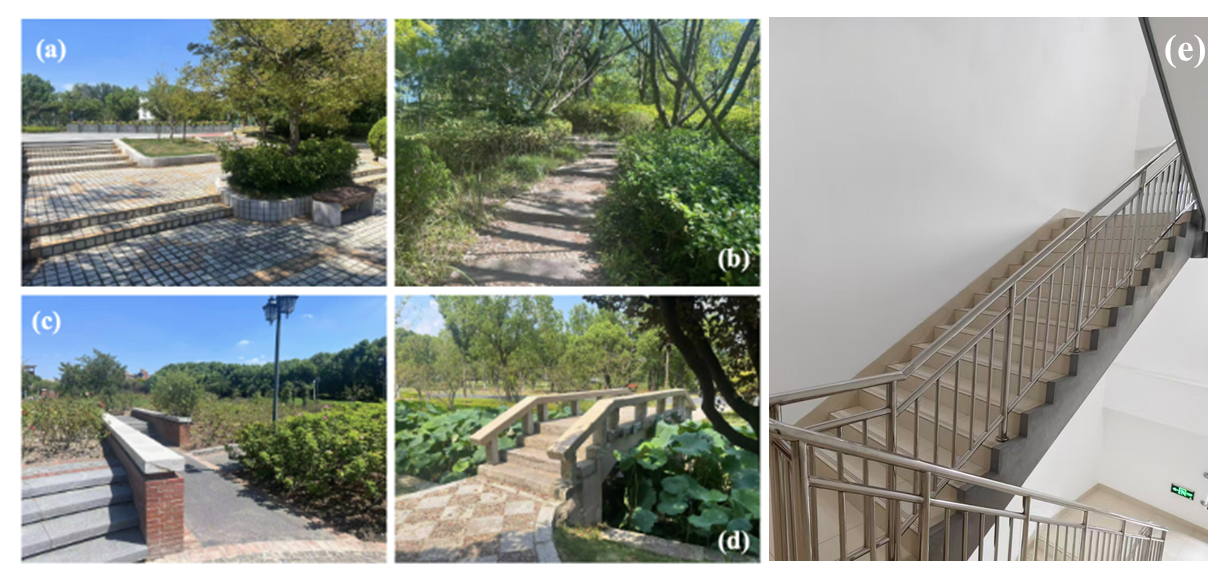
\includegraphics[width=1\linewidth]{figure/map_env/dataset.png}
    \caption{Dataset scenarios: (a) Staircase Scene, (b) Artificial Hill, (c) Rose Garden, (d) Botanical Garden and (e) Indoor Staircase Only. These datasets cover diverse terrain elevations, and each environment contains distinct stair structures for evaluating the $z$-axis localization performance of different methods.}
  \label{fig:dataset-env}
\end{figure}

Due to the lack of publicly available datasets for legged-wheel robots, we collect six datasets in real-world unstructured scenarios that covers a wide variety of indoor and outdoor terrains, surface textures, and elevation profiles.
More specifically, these datasets include abrupt elevation changes, mixed feature densities, and both structured and unstructured environments. 
The scenarios are as follows:
\begin{itemize}
  \item \textbf{Staircase Scene 1 \& 2}: These two sequences traverse flat pavements and different staircases with step heights ranging from 5\,cm to 15\,cm and 1--8 steps, including both single-pass and repeated back-and-forth traversals.
  \item \textbf{Artificial Hill}: This sequence traverses stone-slab paths with multiple single-step stairs, starting from the foot of the hill to the summit, and then returning to the starting point along a different route. It exhibits substantial elevation changes and diverse terrain surface textures.
  \item \textbf{Rose Garden}: This sequence traverses short staircases, flat pavements, and grass slopes, with low lateral obstacles such as flower beds and shrubs. In addition, some staircases are flanked by low walls, which result in sparse geometric features around the staircase region.
  \item \textbf{Botanical Garden}: This sequence covers a long route in the botanical garden, including a suspension bridge, an arch bridge, multiple single-step stairs, and a stone-slab path.
  \item \textbf{Indoor Staircase Only}: This sequence covers a short route that the legged-wheel robot climbs a long indoor stairs. This sequence is mainly used for a stress test for robustness.
\end{itemize}

\textbf{Ground Truth:}
For each sequence (except for ``Indoor Staircase Only"), we additionally record an RTK-corrected position trajectory, including latitude, longitude, and altitude, using the GPS+RTK system. This provides centimeter-level 3D reference trajectories for quantitative evaluation.
We use the RTK-corrected GPS positions as the ground-truth trajectory. However, since the GPS+RTK system provides only latitude, longitude, and altitude, but not orientation, we will evaluate only the translation errors of the compared methods later on.

\subsection{RBF-based Terrain Approximation Result}

In our experiments, we set the mesh resolution of the RBF centers to $0.07\,\mathrm{m}$, the bandwidth parameter $\sigma$ to $0.04\,\mathrm{m}$, and the measurement noise level $\sigma_\epsilon$ to $0.1$. The mesh resolution determines the number of RBF centers and affects both approximation fidelity and computational cost. Empirically, a resolution of $0.07\,\mathrm{m}$ provides sufficient geometric detail for typical terrain variations while maintaining real-time efficiency. The bandwidth parameter $\sigma$ determines the spatial influence of each kernel, while the noise level $\sigma_\epsilon$ accounts for sensor uncertainty and improves robustness to noisy point clouds.

\begin{figure}[!htbp] 
  \centering
  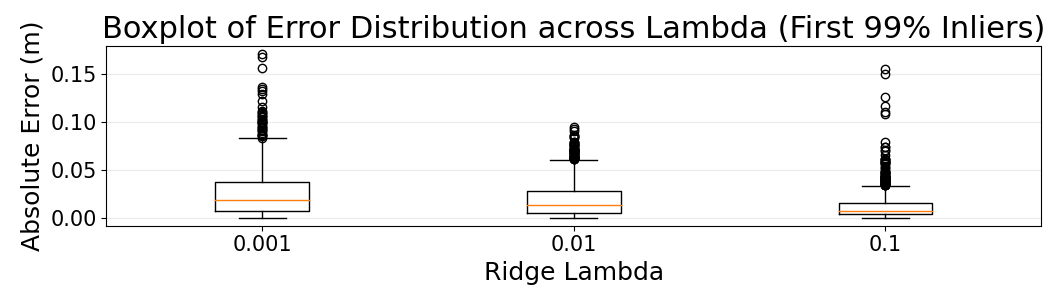
\includegraphics[width=0.95\linewidth]{figure/result/boxplot_lambda.png}
  \caption{Boxplots of the terrain-approximation error for different values of \(\lambda\) on the Rose Garden dataset.}
  \label{fig:boxplot}
\end{figure}

In addition, the ridge penalty parameter \(\lambda\) in ridge regression must be chosen carefully. A too small \(\lambda\) may lead to noise-sensitive and numerically unstable fitting, whereas a too large \(\lambda\) may over-smooth the terrain and blur local geometric details. Therefore, \(\lambda\) should be selected to balance numerical stability and terrain-fitting accuracy. \cs{To evaluate the effect of $\lambda$, we compute the terrain-approximation error using the terrain point cloud observed by the LiDAR. More specifically, at the $k$-th LiDAR frame, let
\begin{equation}
    \mathcal{P}^{\mathrm{ter}}_k
    =
    \left\{
    \mathbf{p}^{i}_k
    =
    \left[
    \left(\mathbf{x}^{i}_k\right)^{\top},
    p^{i}_{z,k}
    \right]^{\top}
    \in \mathbb{R}^{3}
    \right\}^{M_k}_{i=1}
\end{equation}
denote the local terrain points expressed in the world frame after transforming the LiDAR measurements by the estimated robot pose. Here, $\mathbf{x}^{i}_k=[p^{i}_{x,k},p^{i}_{y,k}]^{\top}$ denotes the horizontal coordinate of the $i$-th terrain point, and $p^{i}_{z,k}$ denotes its measured height. For each valid terrain point whose horizontal coordinate lies inside the current RBF region of interest, the approximation error is defined as the absolute vertical residual
\begin{equation}
    e^{i}_k
    =
    \left|
    p^{i}_{z,k}
    -
    f\left(\mathbf{x}^{i}_k;\hat{\mathbf{w}}_k^{RG}\right)
    \right| .
    \label{eq:terrain_approximation_error}
\end{equation}
Therefore, the reported terrain-approximation error measures the consistency between the reconstructed RBF terrain surface and the LiDAR-observed terrain points in the same coordinate frame.}

For the parameter study of $\lambda$, we collect all valid errors $e^{i}_k$ over the Rose Garden sequence and compare their distributions under different ridge penalties. Since LiDAR measurements may contain outliers caused by water-puddle reflections, dynamic objects, or local non-terrain returns, we exclude the top 1\% largest errors when computing the statistics. As shown in Fig.~\ref{fig:boxplot}, $\lambda = 0.001$ leads to larger approximation errors because the regression becomes more sensitive to noise and numerical ill-conditioning, while $\lambda = 0.1$ also increases the error due to excessive smoothing. Therefore, we choose $\lambda = 0.01$, which is used in all subsequent experiments.

\begin{figure}[!htbp]
    \centering
    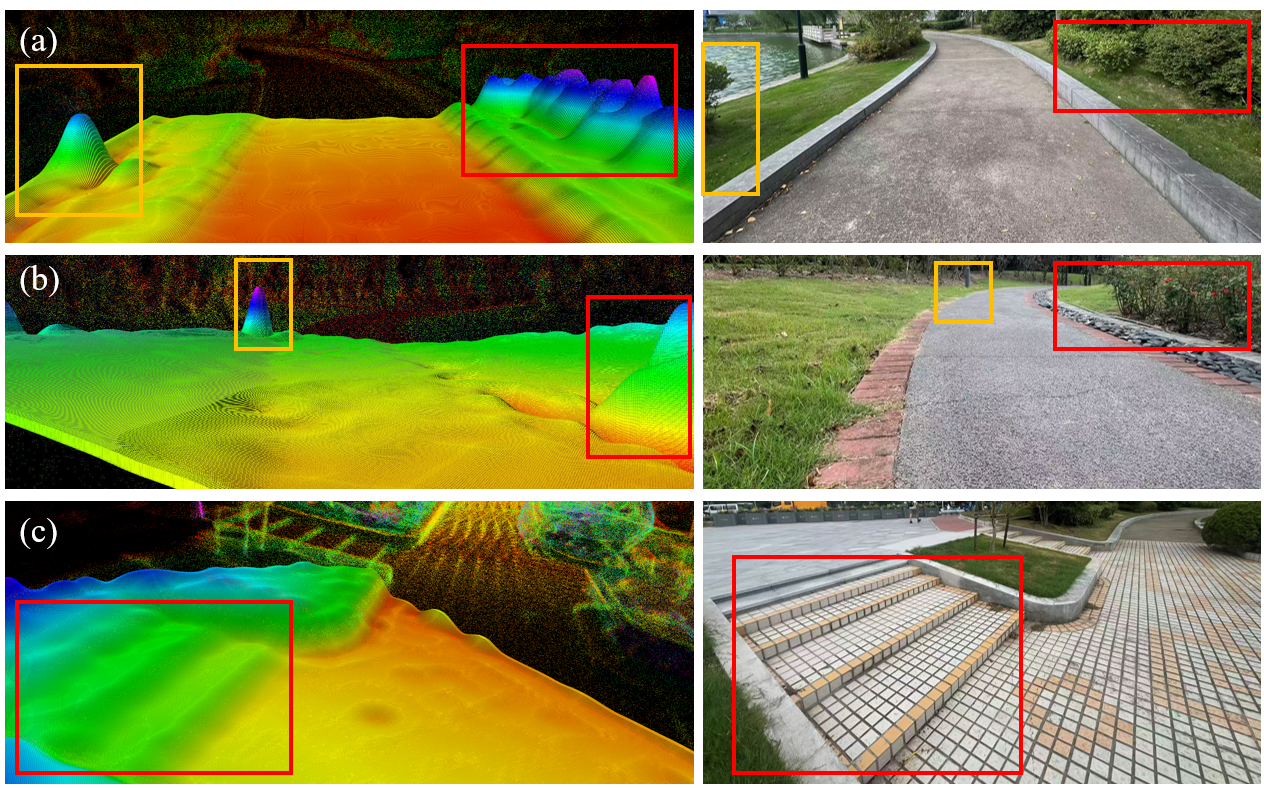
\includegraphics[width=0.9\linewidth]{figure/result/height.png}
    \caption{RBF-based terrain approximation in different environments: (a) flat area, (b) garden pathway, and (c) staircase scene. The colored boxes indicate corresponding objects or local structures across the results.}
    \label{fig:height}
\end{figure}

Next, we qualitatively demonstrate the RBF-based terrain approximation on three representative terrains in Fig.~\ref{fig:height}. In the flat-area scene shown in Fig.~\ref{fig:height}(a), the proposed method reconstructs broad planar regions together with local structures such as bushes and flower beds. In the garden-pathway scene shown in Fig.~\ref{fig:height}(b), the reconstructed terrain captures the local slope variations, the utility pole on the slope, and the boundary between the pathway and the adjacent grass field. In the staircase scene shown in Fig.~\ref{fig:height}(c), the method preserves multiple discrete elevation changes corresponding to individual stair steps.

\begin{figure*}[!htbp]
    \centering
    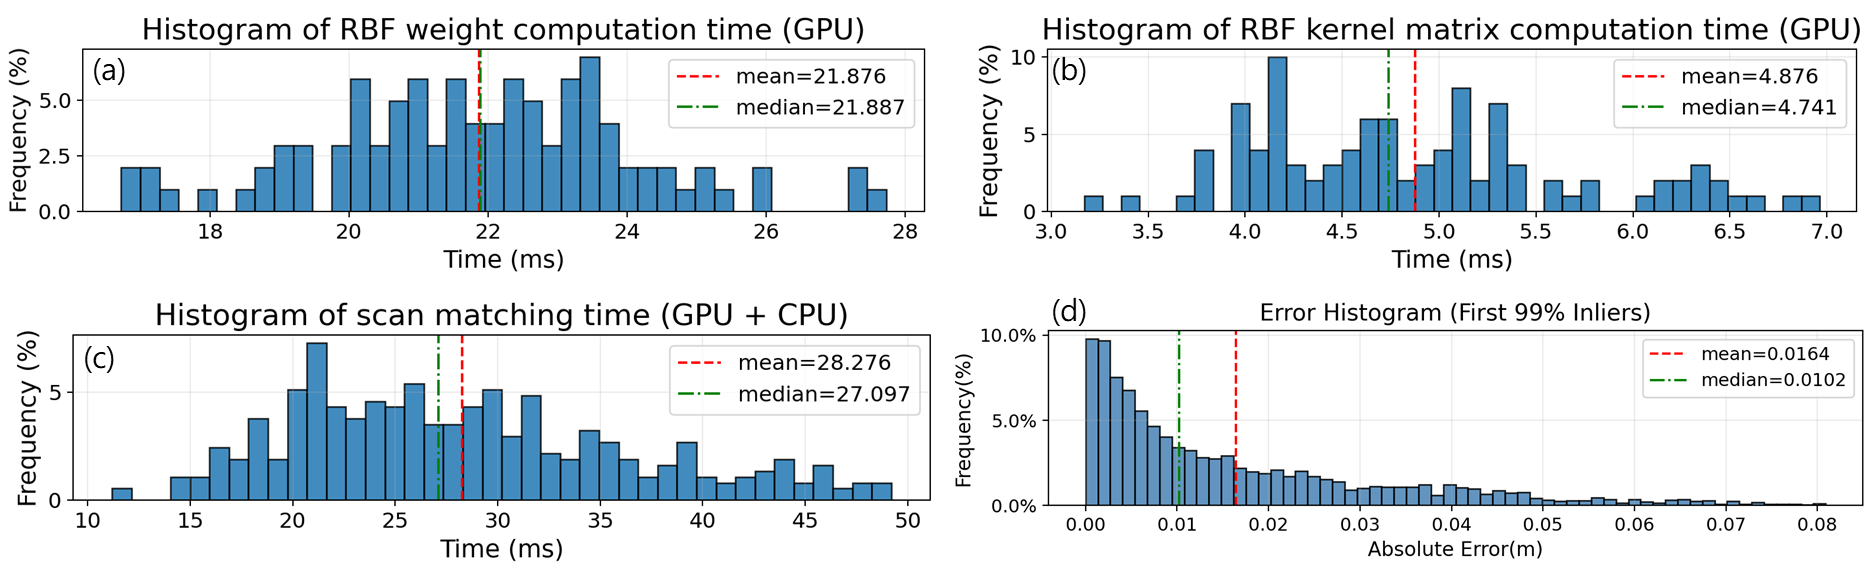
\includegraphics[width=0.92\textwidth]{figure/result/total_hist_0405.png}
    \caption{(a) Histogram of the computation time for RBF weight updates on the GPU. (b) Histogram of the computation time for RBF kernel-matrix evaluation on the GPU. (c) Histogram of the computation time for scan matching on the GPU and CPU. (d) Histogram of the terrain-approximation error on the remaining scenarios in the dataset after excluding the top 1\% outliers.}
    \label{fig:error_height}
\end{figure*}

To further quantify the approximation accuracy, we report the error histogram of the RBF-based terrain approximation in the remaining scenarios of the dataset as shown in Fig.~\ref{fig:error_height}(d).
As a result, under the same evaluation setup, 94.70\% of the errors fall below 0.05\,m. This indicates that the proposed RBF-based terrain approximation achieves good accuracy on terrains with stairs and grass surfaces. This observation is also consistent with the improved localization performance shown later in Fig.~\ref{fig:garden-results}, where RBF-LIO reduces the vertical localization drift that is visible in Fast-LIO2.

Moreover, to demonstrate the real-time performance of the proposed method, we report the computation-time histograms of the main modules in Fig.~\ref{fig:error_height}(a)--(c). The overall framework runs at \SI{10}{\hertz}, which satisfies the real-time requirement of the LiDAR input stream.

\subsection{Ablation Study}

\cs{We conduct three ablation studies to evaluate the main components of the proposed framework. The terrain manifold constraint is evaluated on all sequences with RTK ground truth, while the adaptive center selection and GPU acceleration studies are conducted on the Rose Garden sequence, which contains mixed terrain surfaces and representative height variations. First, we disable the terrain manifold constraint to examine whether the RBF-based wheel--terrain residual contributes to pose estimation. Second, we disable the adaptive RBF center selection strategy to evaluate its influence on terrain-fitting accuracy and online computational cost. Third, we compare the GPU and CPU implementations of the RBF terrain approximation module to quantify the benefit of GPU acceleration. In all ablation experiments, only the target component is changed, while the remaining inputs, parameters, and evaluation settings are kept the same whenever applicable.}

\cs{To verify the contribution of the proposed terrain manifold constraint, we first conduct an ablation study by disabling the manifold residuals in the scan-matching optimization. As shown in Table~\ref{tab:ablation_manifold}, disabling the terrain manifold constraint has only a limited influence on the overall trajectory-wide ATE. This is expected because the scan-matching term still provides the dominant geometric constraint for horizontal motion, and many portions of the trajectories are locally flat or feature-rich. Nevertheless, the proposed manifold constraint consistently reduces the $z$-axis ATE in all evaluated sequences. The improvement is most evident on the Artificial Hill sequence, where the robot continuously traverses slopes and single-step structures, and the $z$-axis ATE is reduced by 27.2\%. These results indicate that the terrain manifold constraint mainly acts as a vertical geometric regularizer rather than a replacement for LiDAR scan matching.}

\begin{table}[!t]
\centering
\caption{\cs{Ablation study of the terrain manifold constraint. Values denote ATE RMSE in meters, and the values in parentheses denote the corresponding $z$-axis ATE RMSE.}}
\label{tab:ablation_manifold}
\footnotesize
\renewcommand{\arraystretch}{1.15}
\setlength{\tabcolsep}{3.0pt}
\begin{tabular}{|c|c|c|c|}
\hline
Sequence & Full RBF-LIO & w/o manifold & $z$-ATE reduction \\
\hline
Staircase 1 & 0.6752 (0.0617) & 0.6715 (0.0682) & 9.5\% \\

Staircase 2 & 0.7858 (0.0625) & 0.7812 (0.0711) & 12.1\% \\

Artificial Hill & 0.4759 (0.1354) & 0.4771 (0.1859) & 27.2\% \\

Rose Garden & 0.5824 (0.1034) & 0.5844 (0.1112) & 7.0\% \\

Botanical Garden & 0.9491 (0.2147) & 0.9435 (0.2275) & 5.6\% \\
\hline
\end{tabular}
\renewcommand{\arraystretch}{1.0}
\end{table}



\cs{Next, we evaluate the adaptive RBF center selection strategy. The full version uses the proposed adaptive center selection strategy, where a candidate RBF center is activated only when it is supported by nearby LiDAR terrain points. The ablated version disables this selection rule and activates all candidate centers inside the current region of interest.}

\begin{table}[!t]
\centering
\caption{\cs{Ablation study of the adaptive RBF center selection strategy on the Rose Garden sequence. The RBF time is the sum of kernel-matrix construction time and weight-update time.}}
\label{tab:ablation_center_selection}
\footnotesize
\renewcommand{\arraystretch}{1.15}
\setlength{\tabcolsep}{2.3pt}
\begin{tabular}{|c|c|c|c|c|}
\hline
Variant & Active centers / ratio & Mean / 95\% error & RBF time \\
\hline
Adaptive centers & 883.8 / 96.0\% & 0.0944 / 0.3414 & 16.88 ms \\

w/o adaptive centers & 920.9 / 100.0\% & 0.0939 / 0.3399 & 19.03 ms \\
\hline
\end{tabular}
\renewcommand{\arraystretch}{1.0}
\end{table}

\cs{As shown in Table~\ref{tab:ablation_center_selection}, compared with the full version, the average number of active centers increases from 883.8 to 920.9. Since more centers are involved in the fitting process, the mean approximation error is only slightly reduced from 0.0944 m to 0.0939 m. However, this small accuracy change is obtained at the cost of higher computation. In particular, the average RBF computation time increases from 16.88 ms to 19.03 ms. Equivalently, the proposed adaptive center selection reduces the RBF computation time by about 11.3\% while maintaining comparable terrain approximation accuracy.}

\cs{Finally, we evaluate the contribution of GPU acceleration to the online RBF terrain approximation. The GPU version uses the CUDA-based implementation for kernel-matrix construction, weight solving, and terrain-height evaluation, while the CPU version performs the same operations on the CPU.}

\begin{table}[!t]
\centering
\caption{\cs{Ablation study of GPU acceleration for online RBF terrain approximation on the Rose Garden sequence. The total RBF time is the sum of kernel-matrix construction time, weight-solving time, and terrain-evaluation time.}}
\label{tab:ablation_gpu_acceleration}
\footnotesize
\renewcommand{\arraystretch}{1.15}
\setlength{\tabcolsep}{1.8pt}
\begin{tabular}{|c|c|c|c|c|c|}
\hline
Variant & Mean / 95\% error & Kernel & Weight & Eval. & Total \\
\hline
GPU & 0.1176 / 0.4103 & 2.08 ms & 15.53 ms & 4.56 ms & 22.17 ms \\

CPU & 0.1161 / 0.4057 & 98.67 ms & 4339.21 ms & 69.04 ms & 4506.92 ms \\
\hline
\end{tabular}
\renewcommand{\arraystretch}{1.0}
\end{table}

\cs{As shown in Table~\ref{tab:ablation_gpu_acceleration}, the GPU and CPU implementations achieve comparable terrain approximation accuracy. In terms of runtime, the GPU implementation significantly reduces the computational cost of all RBF-related operations. The kernel-matrix construction time decreases from 98.67 ms to 2.08 ms, the weight-solving time decreases from 4339.21 ms to 15.53 ms, and the total RBF computation time decreases from 4506.92 ms to 22.17 ms. This result demonstrates that GPU acceleration is essential for maintaining online terrain reconstruction in the proposed RBF-LIO framework.}

\subsection{Robustness to Degraded Terrain Observations}
\label{subsec:terrain_observation_stress}

\cs{To examine whether the RBF terrain representation relies heavily on dense ground observations from the inverted LiDAR, we conduct a controlled stress test on the Rose Garden sequence. Before RBF fitting, the terrain point cloud is degraded in four settings: full observations, random sparsification with 50\% and 25\% retained points, and sector occlusion by removing points within a forward-facing $60^{\circ}$ angular sector. The RBF model is fitted using the degraded observations, while the validation error is computed on the original full terrain point cloud of the same frame.}

\cs{As shown in Table~\ref{tab:terrain_observation_stress}, all settings maintain a valid-frame ratio of 100\%. Random sparsification reduces the average number of active centers from 744.6 to 691.2 and 616.9, confirming that the terrain support is effectively reduced. Nevertheless, the full-cloud validation errors remain close to the full-observation setting. The sector-occlusion setting shows a similar trend. These results indicate that the RBF terrain approximation remains stable under moderate sparsification and partial field-of-view reduction, as long as sufficient local terrain support is available.}

\begin{table}[!t]
\centering
\caption{\cs{Robustness test under degraded terrain observations on the Rose Garden sequence. The full-cloud validation error is computed on the original full terrain point cloud of the same frame. Error values denote mean / 95\% vertical residuals in meters.}}
\label{tab:terrain_observation_stress}
\footnotesize
\renewcommand{\arraystretch}{1.15}
\setlength{\tabcolsep}{3.0pt}
\begin{tabular}{|c|c|c|c|c|}
\hline
Setting & Kept ratio & Valid frames & Active centers & Full-val. error \\
\hline
Full & 100.0\% & 100.0\% & 744.6 & 1.5147 / 4.3010 \\

Sparse 50\% & 50.0\% & 100.0\% & 691.2 & 1.5492 / 4.3473 \\

Sparse 25\% & 25.0\% & 100.0\% & 616.9 & 1.4944 / 4.2071 \\

Sector occ. & 92.7\% & 100.0\% & 658.0 & 1.5026 / 4.2180 \\
\hline
\end{tabular}
\renewcommand{\arraystretch}{1.0}
\end{table}

\subsection{Comparison Results}
Our proposed RBF-LIO is evaluated against five representative baselines: Fast-LIO2 \cite{fastlio2}, ROLO-SLAM \cite{roloslam}, Leg-KILO \cite{leg-kilo}, GLIM \cite{glim}, and Wheel-Legged SLAM \cite{wl-slam}. In particular, Fast-LIO2 and GLIM have demonstrated strong localization and mapping performance on ground vehicles and aerial platforms. In contrast, ROLO-SLAM, Leg-KILO, and Wheel-Legged SLAM are more closely related to our setting, since they are designed to mitigate $z$-axis pose drift. Although Leg-KILO and Wheel-Legged SLAM were originally developed for quadruped robots, their core mechanisms of incorporating kinematic constraints into LiDAR--inertial odometry are general. To ensure a fair comparison, we adapt these baselines to our legged-wheel platform. Specifically, we provide the requisite leg-joint kinematics for both Leg-KILO and Wheel-Legged SLAM. In addition, Leg-KILO's contact model is permanently activated to reflect the continuous wheel--terrain contact, while for GLIM, only its odometry module is used. Moreover, at the beginning of each experiment, the robot remains stationary for a period of time to complete state initialization.

\cs{To make the comparison protocol explicit, Table~\ref{tab:baseline_inputs} summarizes the sensor measurements and additional geometric information used by each method. We do not modify LiDAR--IMU-only baselines to use joint measurements or terrain contact information, because doing so would change their original algorithmic assumptions and require designing new factors that are outside the scope of those methods. Therefore, Fast-LIO2, GLIM, and ROLO-SLAM are used as representative general-purpose odometry baselines, while Leg-KILO and Wheel-Legged SLAM are used as more closely related kinematic/contact-aware baselines.}

\begin{table*}[!t]
\centering
\caption{\cs{Sensor measurements and additional geometric information used by each method in the comparison.}}
\label{tab:baseline_inputs}
\small
\renewcommand{\arraystretch}{1.15}
\setlength{\tabcolsep}{5.0pt}
\begin{tabular}{|p{0.2\textwidth}|c|c|c|p{0.27\textwidth}|p{0.21\textwidth}|}
\hline
Method & LiDAR & IMU & Joint sensors & Kinematic/contact information & Explicit terrain model \\
\hline
Fast-LIO2~[1] & Yes & Yes & No & No & No \\

GLIM~[2] & Yes & No & No & No & No \\

ROLO-SLAM~[4] & Yes & No & No & Rotation constraint & No \\

Leg-KILO~[3] & Yes & Yes & Yes & Leg kinematics and local contact plane & Local planar model \\

Wheel-Legged SLAM~[5] & Yes & Yes & Yes & Wheel-leg kinematics & Local contact constraint \\

RBF-LIO (ours) & Yes & Yes & Yes & Wheel--terrain contact geometry & Online RBF terrain manifold \\
\hline
\end{tabular}
\renewcommand{\arraystretch}{1.0}
\end{table*}

\cs{In addition, we keep the following settings the same in all comparisons:
\begin{itemize}
\item \textbf{Dataset and synchronization:} All methods are evaluated on the same rosbag sequences and use the same LiDAR scans recorded by the inverted Mid360 LiDAR(\SI{10}{\hertz}). Methods that use IMU measurements are provided with the same Mid360 IMU topic(\SI{200}{\hertz}), and methods that use robot kinematics are provided with the same joint-sensor topic(\SI{500}{\hertz}).
\item \textbf{Initialization:} At the beginning of each experiment, the robot remains stationary for a short period to allow state initialization. The same initialization segment is used for all methods.
\item \textbf{Preprocessing and resolution:} The same voxel resolution of 0.2 m is used for LiDAR down-sampling in scan matching. The same LiDAR frame range and evaluation interval are used when computing the trajectory errors.
\item \textbf{IMU parameters:} For the methods that use IMU measurements, the noise covariance matrices for linear acceleration and angular velocity are set to $10^{-2}I_3$, while the corresponding bias covariance matrices are set to $10^{-4}I_3$.
\item \textbf{Evaluation metric:} Since the GPS+RTK system provides only position measurements without orientation, all methods are evaluated using translation errors only. The same RTK trajectory, time association, and alignment protocol are used for all quantitative comparisons.
\end{itemize}}

\begin{figure*}[!htpb]
    \centering
    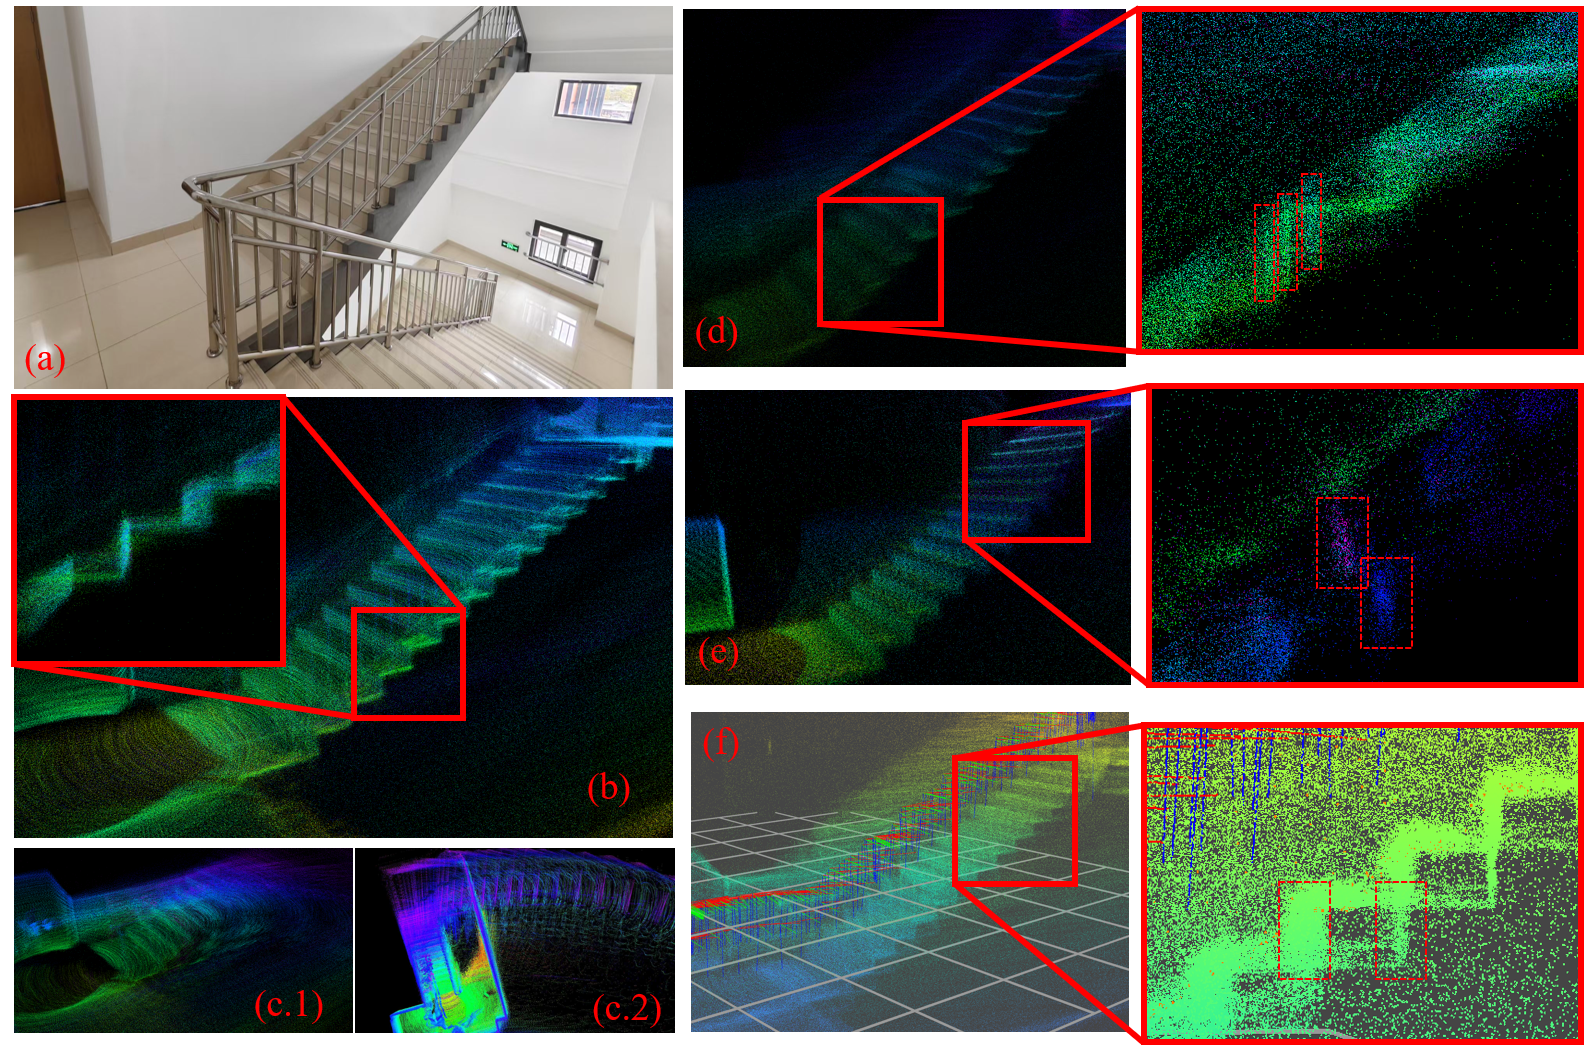
\includegraphics[width=0.9\textwidth]{figure/traj/new_stair_drift.png}
    \caption{Qualitative comparison of point cloud maps generated in an indoor staircase-only scenario. (a) Reference photograph of the environment. Mapping results produced by (b) RBF-LIO, (c.1) Wheel-Legged SLAM, (c.2) top view of Wheel-Legged SLAM, (d) FAST-LIO2, (e) Leg-KILO, and (f) GLIM. The zoomed-in views highlight the staircase structure reconstructed by each method. The dashed red rectangles indicate the same vertical plane of a single step for visual comparison.}
    \label{fig:stair_drift}
\end{figure*}

We first examine a staircase-only indoor scenario to highlight the robustness of the compared methods under abrupt elevation changes. As shown in Fig.~\ref{fig:stair_drift}, RBF-LIO produces a structurally consistent point cloud map of the staircase. In contrast, the maps generated by the other methods exhibit varying degrees of ghosting and layering artifacts, suggesting reduced robustness under repeated abrupt elevation changes. This experiment serves as a stress test and directly illustrates the advantage of explicitly incorporating terrain geometry in environments dominated by abrupt height transitions.

We further qualitatively evaluate the compared methods on our collected datasets.
The improvements are indeed most visible along the vertical dimension.
\begin{figure}[!htbp] 
  \centering
  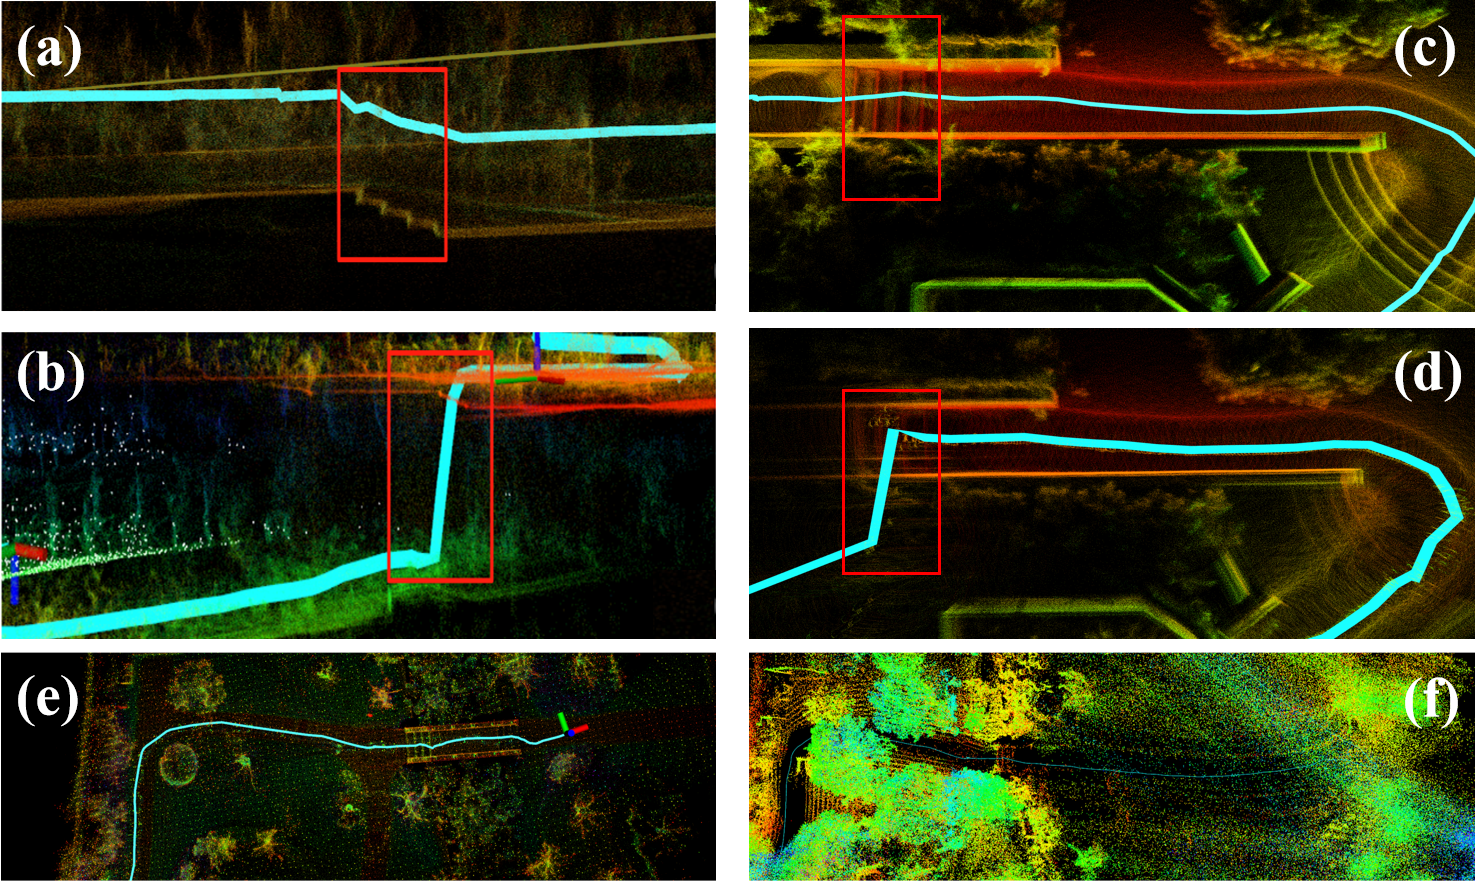
\includegraphics[width=0.95\linewidth]{figure/traj/drift_new.png}
  \caption{Visualization of the mapping results: (a) RBF-LIO on the Rose Garden dataset, (b) Fast-LIO2 on the Rose Garden dataset, (c) RBF-LIO on a staircase in a feature-rich environment, (d) Wheel-Legged SLAM in the same environment as (c), (e) RBF-LIO on the Botanical Garden dataset, and (f) Leg-KILO on the Botanical Garden dataset.}
  \label{fig:garden-results}
\end{figure}
As illustrated in Fig.~\ref{fig:garden-results}, Fast-LIO2 suffers from pose drift and map layering artifacts in Rose Garden, where sparse features and abrupt elevation changes occur simultaneously. Moreover, on the same staircase in Rose Garden, Wheel-Legged SLAM incorrectly fits the plane and fails to map. In addition, in the Botanical Garden dataset, where the terrain is more complex, Leg-KILO suffers from pose drift, which is consistent with the limitation of its coarse terrain model. Although kinematic constraints can improve estimation in feature-sparse environments, the local flatness assumption in Leg-KILO is likely to be violated by uneven structures such as the suspension bridge and the arch bridge, while the reduced geometric richness may further degrade plane extraction. In contrast, RBF-LIO continuously corrects the height estimate through the manifold soft constraints, thereby preserving a more globally consistent map.

Furthermore, we compare the trajectories in Rose Garden. We choose this scenario as a representative one because it contains sparse features together with abrupt height changes. In particular, Fast-LIO2 and Wheel-Legged SLAM both diverge, while the pose estimation error of ROLO-SLAM is too large. Therefore, the trajectories of these three methods are not depicted in Fig.~\ref{fig:traj}. 
\begin{figure}[!htpb]
    \centering
    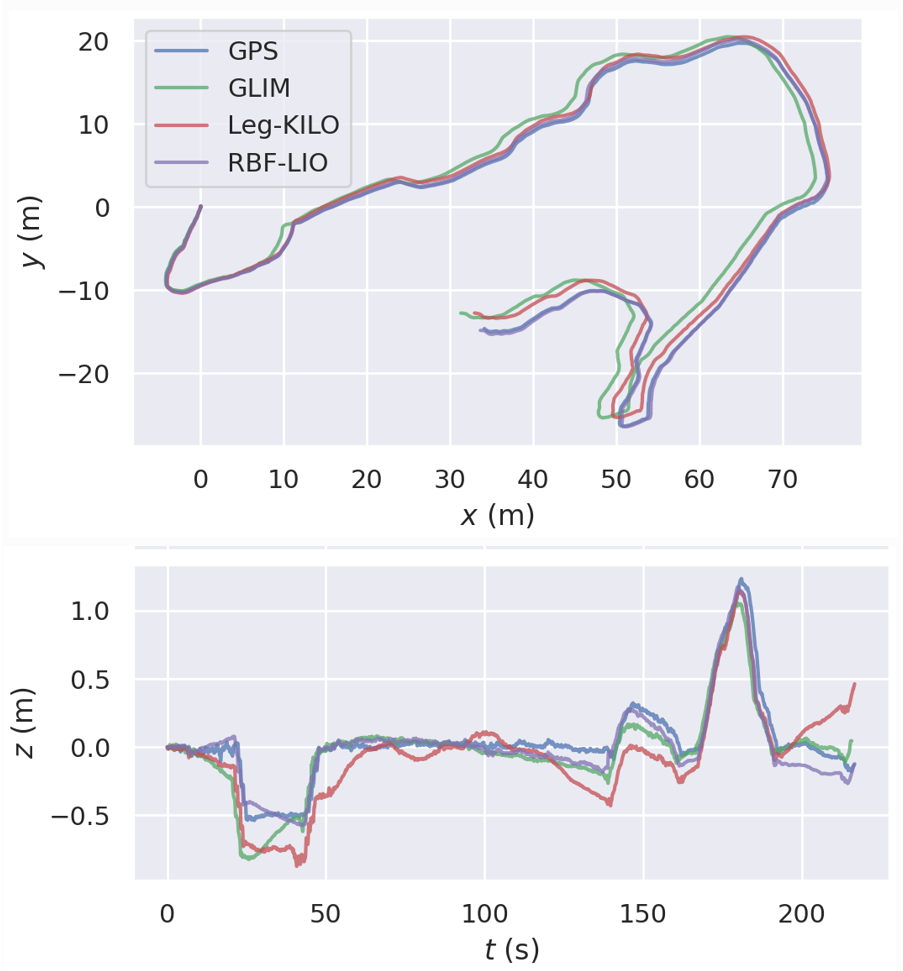
\includegraphics[width=0.9\linewidth]{figure/traj/new_garden_xy_plus_z.png}
    \caption{Trajectories of different methods on the Rose Garden dataset: projection on the \(xoy\)-plane and evolution along the \(z\)-axis.}
    \label{fig:traj}
\end{figure}
As shown in Fig.~\ref{fig:traj}, Leg-KILO and GLIM exhibit noticeable z-axis drift, whereas RBF-LIO maintains the closest alignment with the RTK reference.

Next, we quantitatively compare the performance of RBF-LIO with the baselines. In particular, we report the Absolute Trajectory Error (ATE) and Relative Trajectory Error (RTE) of all methods in Table.~\ref{tab:ape} and Table.~\ref{tab:rpe}. In addition to the overall trajectory errors, we also report the errors of the $z$ component in parentheses to directly evaluate the effect of the proposed manifold soft constraints on vertical localization. The best results are highlighted in bold font.


\begin{table*}[!htpb]
\centering
\setlength{\tabcolsep}{3pt}
\scriptsize
\caption{ATE\cite{ATE} (m) for different methods. Values in parentheses denote $z$-axis errors. Slash means failure.}
\label{tab:ape}

\makebox[\textwidth][c]{%
\resizebox{\textwidth}{!}{%
\begin{tabular}{|C{1.3cm}|C{0.95cm}C{0.95cm}|C{0.95cm}C{0.95cm}|C{0.95cm}C{0.95cm}|C{0.9cm}C{0.9cm}|C{0.9cm}C{0.9cm}|C{0.9cm}C{0.9cm}|}
\hline
Sequence
& \multicolumn{2}{c|}{RBF-LIO}
& \multicolumn{2}{c|}{\makecell{Fast-LIO2\\\cite{fastlio2}}}
& \multicolumn{2}{c|}{\makecell{ROLO-SLAM\\\cite{roloslam}}}
& \multicolumn{2}{c|}{\makecell{Leg-KILO\\\cite{leg-kilo}}}
& \multicolumn{2}{c|}{GLIM\cite{glim}}
& \multicolumn{2}{c|}{\makecell{Wheel-Legged \\SLAM\cite{wl-slam}}} \\
\cline{2-13}
& \multicolumn{1}{c|}{RMSE} & \multicolumn{1}{c|}{max}
& \multicolumn{1}{c|}{RMSE} & \multicolumn{1}{c|}{max}
& \multicolumn{1}{c|}{RMSE} & \multicolumn{1}{c|}{max}
& \multicolumn{1}{c|}{RMSE} & \multicolumn{1}{c|}{max}
& \multicolumn{1}{c|}{RMSE} & \multicolumn{1}{c|}{max}
& \multicolumn{1}{c|}{RMSE} & \multicolumn{1}{c|}{max} \\
\hline
Staircase 1
& 0.6752 (0.0617) & 1.3126 (0.3588)
& 0.7471 (\textbf{0.0587}) & 1.4464 (\textbf{0.3166})
& 21.6712 (1.0336) & 29.2766 (2.4170)
& \textbf{0.6347} (0.0615) & \textbf{1.1855} (0.3393)
& 0.7357 (0.1793) & 1.3265 (0.4787)
& 1.4982 (0.3200) & 2.5845 (0.7898) \\
Staircase 2
& \textbf{0.7858} (\textbf{0.0625}) & \textbf{1.2764} (0.3372)
& 0.9039 (0.0670) & 1.5034 (\textbf{0.3207})
& 36.7933 (3.8083) & 65.8538 (9.8349)
& 0.8160 (0.0832) & 1.5232 (0.3841)
& 0.9872 (0.2074) & 1.7557 (0.5310)
& 1.5265 (0.2032) & 3.6606 (0.5622) \\
Artificial Hill
& 0.4759 (\textbf{0.1354}) & 0.9555 (\textbf{0.5144})
& 0.6088 (0.1553) & 1.1251 (0.5210)
& 16.1785 (6.4400) & 24.1648 (11.2143)
& \textbf{0.4534} (0.1394) & \textbf{0.8362} (0.5162)
& 0.6190 (0.2300) & 1.1597 (0.6370)
& 1.8872 (0.3987) & 3.3049 (1.0807) \\
Rose Garden
& \textbf{0.5824} (0.1034) & \textbf{1.0972} (\textbf{0.2628})
& /\ & /\
& 16.9995 (1.5915) & 27.4158 (4.8372)
& 0.9069 (0.1669) & 1.8861 (0.6708)
& 1.2513 (\textbf{0.0965}) & 2.1290 (0.3550)
& /\ & /\ \\
Botanical Garden
& \textbf{0.9491} (0.2147) & \textbf{1.6648} (0.4915)
& 1.2962 (0.3683) & 4.0772 (1.2227)
& 22.3889 (3.3272) & 41.6459 (7.2956)
& /\ & /\
& 0.9980 (\textbf{0.1595}) & 1.8093 (\textbf{0.4791})
& 2.6237 (0.3509) & 4.5260 (0.8286) \\
\hline
\end{tabular}%
}%
}
\normalsize
\end{table*}

\begin{table*}[!htpb]
\centering
\setlength{\tabcolsep}{3pt}
\scriptsize
\caption{RTE\cite{ATE} (m) ($\Delta t=0.1\,\mathrm{s}$) for different methods. Values in parentheses denote $z$-axis errors. Slash means failure.}
\label{tab:rpe}

\makebox[\textwidth][c]{%
\resizebox{\textwidth}{!}{%
\begin{tabular}{|C{1.3cm}|C{0.95cm}C{0.95cm}|C{0.95cm}C{0.95cm}|C{0.95cm}C{0.95cm}|C{0.9cm}C{0.9cm}|C{0.9cm}C{0.9cm}|C{0.9cm}C{0.9cm}|}
\hline
Sequence
& \multicolumn{2}{c|}{RBF-LIO}
& \multicolumn{2}{c|}{\makecell{Fast-LIO2\\\cite{fastlio2}}}
& \multicolumn{2}{c|}{\makecell{ROLO-SLAM\\\cite{roloslam}}}
& \multicolumn{2}{c|}{\makecell{Leg-KILO\\\cite{leg-kilo}}}
& \multicolumn{2}{c|}{GLIM\cite{glim}}
& \multicolumn{2}{c|}{\makecell{Wheel-Legged SLAM\\\cite{wl-slam}}} \\
\cline{2-13}
& \multicolumn{1}{c|}{RMSE} & \multicolumn{1}{c|}{max}
& \multicolumn{1}{c|}{RMSE} & \multicolumn{1}{c|}{max}
& \multicolumn{1}{c|}{RMSE} & \multicolumn{1}{c|}{max}
& \multicolumn{1}{c|}{RMSE} & \multicolumn{1}{c|}{max}
& \multicolumn{1}{c|}{RMSE} & \multicolumn{1}{c|}{max}
& \multicolumn{1}{c|}{RMSE} & \multicolumn{1}{c|}{max} \\
\hline
Staircase 1
& 0.0503 (0.0170) & \textbf{0.2267} (0.1333)
& 0.0556 (0.0124) & 0.2546 (0.1058)
& 0.1694 (0.0401) & 1.1933 (0.3205)
& \textbf{0.0478} (0.0124) & 0.2344 (0.1064)
& 0.0545 (0.0232) & 0.4161 (0.4037)
& 0.1073 (\textbf{0.0108}) & 0.7914 (\textbf{0.0968}) \\
Staircase 2
& 0.0493 (0.0138) & \textbf{0.2227} (\textbf{0.0758})
& 0.0493 (0.0148) & 0.2333 (0.1006)
& 0.2027 (0.0650) & 0.8776 (0.3859)
& \textbf{0.0461} (0.0141) & 0.2294 (0.1095)
& 0.0480 (0.0140) & 0.2257 (0.1025)
& 0.0869 (\textbf{0.0113}) & 0.8077 (0.0779) \\
Artificial Hill
& \textbf{0.0277} (0.0314) & \textbf{0.4614} (\textbf{0.4198})
& 0.0864 (0.0365) & 0.5699 (0.4227)
& 0.3977 (0.0993) & 8.7865 (0.7038)
& 0.0605 (\textbf{0.0301}) & 0.4617 (0.4434)
& 0.0624 (0.0305) & 0.4645 (0.4478)
& 0.1233 (0.0336) & 1.1333 (0.4536) \\
Rose Garden
& \textbf{0.0363} (0.0154) & \textbf{0.1744} (0.0979)
& /\ & /\
& 0.1881 (0.0530) & 0.6960 (0.2968)
& 0.0595 (0.0114) & 0.2337 (\textbf{0.0860})
& 0.0413 (\textbf{0.0113}) & 0.2288 (0.1415)
& /\ & /\ \\
Botanical Garden
& 0.0849 (0.0179) & 0.3815 (0.3343)
& 0.0664 (0.0197) & 0.5346 (0.3514)
& 0.2104 (0.0639) & 0.8683 (\textbf{0.3172})
& /\ & /\
& \textbf{0.0575} (0.0185) & \textbf{0.3550} (0.3472)
& 0.0938 (\textbf{0.0168}) & 0.7006 (0.3530) \\
\hline
\end{tabular}%
}
}

\normalsize
\end{table*}


Both GLIM and RBF-LIO succeed in estimating the poses on all datasets.
In scenarios with rich geometric features but abrupt height changes, such as Artificial Hill and Staircase Scene 1 \& 2, the ATE of RBF-LIO is generally comparable to that of the strongest competing methods. This suggests that, in feature-rich environments, the baselines can maintain comparable overall trajectory accuracy. However, as the terrain becomes more complex, the difference between the methods becomes more evident. Moreover, RBF-LIO also outperforms ROLO-SLAM, which is explicitly designed to reduce vertical errors.

Notably, the improvement in RTE is less pronounced than that in ATE. This is consistent with the different roles of the two metrics: RTE evaluates short-horizon local consistency over a fixed interval, whereas ATE reflects the accumulated global drift over the entire trajectory. Since the proposed manifold constraints mainly take effect when the robot traverses abrupt elevation transitions such as stairs, their benefit is diluted in trajectory-wide RTE statistics that average over many locally easy segments. In contrast, the suppression of vertical drift accumulates over time and is therefore more clearly reflected in ATE, especially in the $z$-axis error.

To summarize, both the quantitative and qualitative results show that the proposed RBF-LIO offers a more robust performance in scenarios that have abrupt elevation changes than the baselines. In particular, the advantage of RBF-LIO is most evident in its suppression of accumulated vertical drift and its ability to preserve global consistency in challenging terrain, yet still performs comparably well on normal terrain.

\subsection{Wet-Grass Stress Test}
\label{subsec:wet_grass_stress}

\cs{To evaluate the behavior of RBF-LIO under slippery-surface and contact-uncertain conditions, we collect an additional wet-grass sequence after rain using the same sensor configuration as the other outdoor sequences. We compare the full RBF-LIO with Fast-LIO2, GLIM, and RBF-LIO without the terrain manifold constraint.}

\begin{figure}[!htpb]
    \centering
    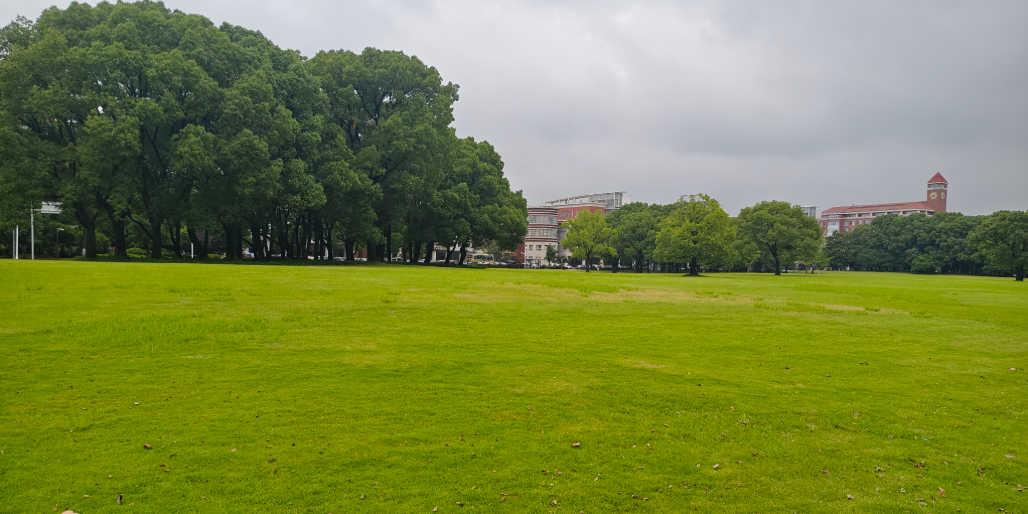
\includegraphics[width=0.9\linewidth]{figure/map_env/wet_grass.png}
    \caption{Wet-grass scenario.}
    \label{fig:traj}
\end{figure}

\cs{As shown in Table~\ref{tab:wet_grass_stress}, all methods complete the sequence without divergence. RBF-LIO achieves the lowest ATE and z-ATE. Compared with the ablated version without the terrain manifold constraint, the full method reduces the z-ATE from 0.1850 m to 0.1442 m, corresponding to a relative reduction of about 22.1\%. The RTE values of the full and ablated variants are close, indicating that the manifold constraint improves vertical consistency without degrading short-term odometry stability.}

\cs{This stress test also illustrates the limitation of contact-based terrain constraints. On slippery or deformable surfaces, wheel--terrain contact may become unreliable. Therefore, the manifold term is used as a soft residual rather than a hard constraint. When large manifold residuals, insufficient terrain support, abnormal RBF fitting errors, or sudden IMU changes are detected, the constraint can be down-weighted or disabled, allowing the estimator to fall back to LiDAR--IMU scan matching.}

\begin{table}[!t]
\centering
\caption{\cs{Wet-grass stress test under a slippery-surface condition. ATE, $z$-ATE, and RTE are reported in meters.}}
\label{tab:wet_grass_stress}
\footnotesize
\renewcommand{\arraystretch}{1.15}
\setlength{\tabcolsep}{12.0pt}
\begin{tabular}{|c|c|c|c|}
\hline
Method & ATE & $z$-ATE & RTE \\
\hline
Fast-LIO2 & 0.8836 & 0.2248 & 0.068 \\

GLIM & 0.7911 & 0.1712 & 0.059 \\

RBF-LIO w/o manifold & 0.7654 & 0.1850 & 0.054 \\

RBF-LIO & 0.7023 & 0.1442 & 0.055 \\
\hline
\end{tabular}
\renewcommand{\arraystretch}{1.0}
\end{table}

% \FloatBarrier

\subsection{Cross-Platform Staircase Stress Test}
\label{subsec:m20_cross_platform}

\cs{We further conduct a qualitative cross-platform staircase test on a DeepRobotics Lynx M20 four-wheel-legged robot. Unlike the Tron1 platform used in the main experiments, the M20 uses a front-facing LiDAR configuration, which provides less favorable and less uniform ground observations than the inverted Mid360 setup. The selected half-floor staircase segment contains 183 poses over 36.40 s, with a trajectory length of 12.03 m and an elevation range of 2.23 m.}

\cs{As shown in Fig.~\ref{fig:m20_staircase_map}, RBF-LIO generates a continuous staircase map on the M20 platform. Compared with the Tron1 results, the reconstructed map contains more local noise and thickness, which is mainly caused by the front-facing LiDAR and sparser ground observations. Nevertheless, the staircase structure remains recognizable and the mapping process does not diverge. In contrast, Leg-KILO produces a blurred and thick staircase map, while Wheel-Legged SLAM fails to preserve a consistent staircase structure and exhibits severe trajectory drift. This provides qualitative evidence that the LiDAR--inertial and terrain-aware mapping pipeline can operate on a different wheel-legged platform and LiDAR mounting configuration.}

\cs{Since the M20 platform differs from Tron1 in morphology, LiDAR mounting, ground-observation density, and wheel--terrain contact geometry, a complete transfer of the full manifold constraint requires platform-specific kinematic parameters and contact-reliability checks. More generally, the proposed manifold constraint assumes reliable wheel--terrain contact, sufficient local terrain support, and a terrain surface that can be locally represented as a single-valued height function. These assumptions may be weakened near sharp stair edges, highly deformable grass, severe wheel slip, temporary loss of contact, strong vibration, or multi-layer structures. In such cases, the manifold residual should be down-weighted or rejected, allowing the estimator to rely on the LiDAR--IMU scan-matching objective.}

\begin{figure*}[!t]
\centering
\begin{minipage}{0.31\textwidth}
\centering
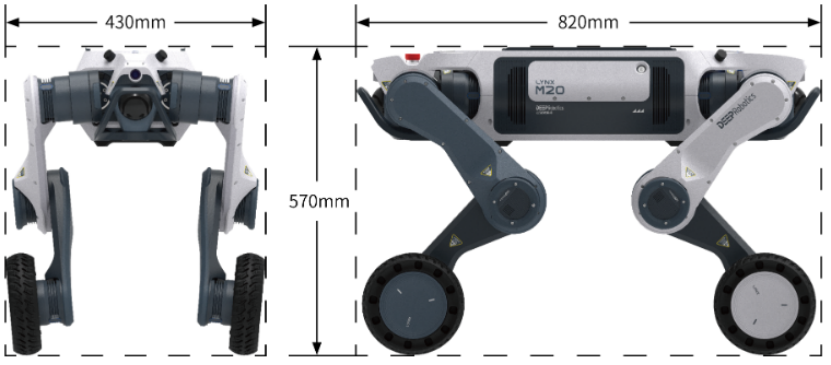
\includegraphics[width=\linewidth]{figure/robot_setting/m20.png}\\
\footnotesize (a) Robot platform
\end{minipage}
\hfill
\begin{minipage}{0.68\textwidth}
\centering
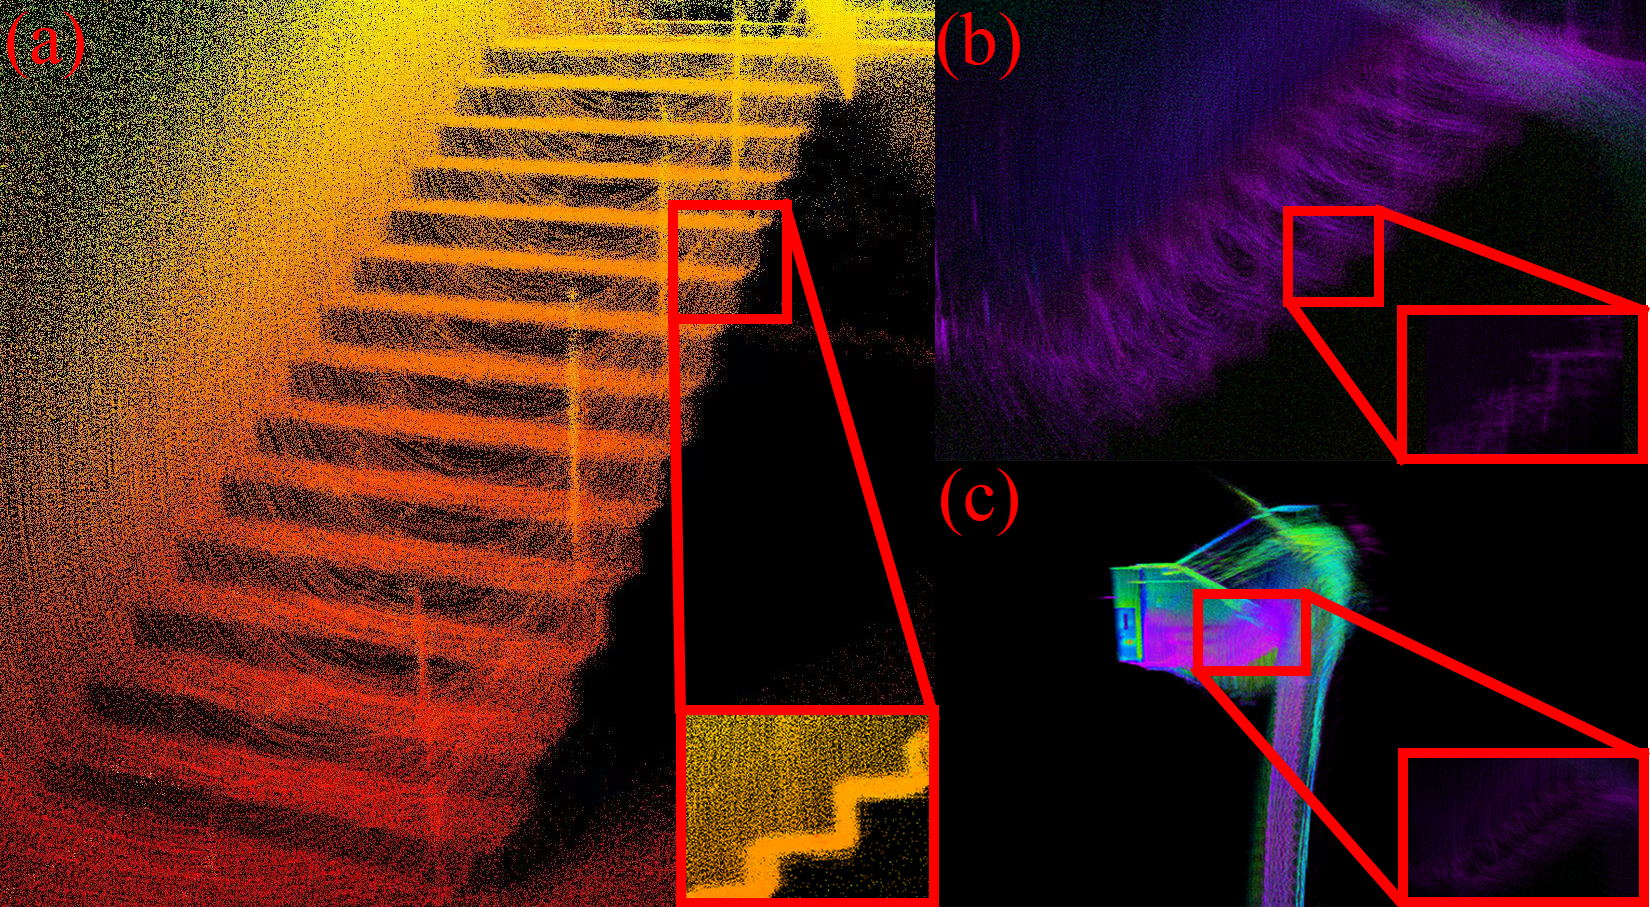
\includegraphics[width=\linewidth]{figure/traj/m20_stair_drift3.png}\\
\footnotesize (b) Side and zoomed-in views. The mapping results are produced by (a) RBF-LIO, (b) Leg-KILO, and (c) Wheel-Legged SLAM, respectively.
\end{minipage}
\caption{\cs{Qualitative cross-platform staircase stress test on the M20 four-wheel-legged robot. The LiDAR is mounted in a front-facing configuration, which provides less favorable ground observations than the inverted Mid360 setup used on the Tron1 platform. In the zoomed-in comparison, RBF-LIO preserves a clearer staircase structure, Leg-KILO produces a blurred and thick map, and Wheel-Legged SLAM suffers from severe drift.}}
\label{fig:m20_staircase_map}
\end{figure*}

\section{Conclusion}
In this paper, we proposed RBF-LIO, a LiDAR--inertial odometry framework that incorporates terrain constraints to improve vertical localization accuracy. In particular, the terrain is approximated by radial basis functions (RBFs) based on moment conditions, and the resulting estimation problem is further reformulated as a recursive ridge regression problem. This yields a smooth terrain manifold, which is then introduced into the gradient-based LIO optimization as a set of soft constraints to mitigate localization errors along the $z$-axis.
Experimental results demonstrate that the proposed method significantly suppresses $z$-axis pose drift in environments with large height differences and abrupt elevation changes, compared with state-of-the-art methods. As a result, the introduced soft constraints enable continuous height correction in the LIO framework, thereby producing coherent and high-fidelity maps even in staircase scenarios and feature-sparse environments.
Moreover, we release a dataset to support future SLAM research on legged-wheel robots.

% References

\bibliographystyle{IEEEtran}
\bibliography{refs}
	
\end{document}
